\documentclass[11pt, a4paper]{report}   	% use "amsart" instead of "article" for AMSLaTeX format

\usepackage{geometry}
\usepackage[parfill]{parskip}    		% Activate to begin paragraphs with an empty line rather than an indent
\usepackage{graphicx}				% Use pdf, png, jpg, or eps with pdflatex; use eps in DVI mode
\usepackage[english, american]{babel}
\usepackage{csquotes}
\usepackage{xr} % Fross cross-referencing between multiple tex-files
\usepackage{caption} % Removes [:] in figure captions
\usepackage{placeins}
\usepackage[utf8]{inputenc}
\usepackage{amssymb}
\usepackage{amsmath}
\usepackage{bm}
\usepackage{amsthm}
\usepackage{stmaryrd}
\usepackage{verbatim}
\usepackage{enumerate} % Pretty lists with (i),(ii)...
\usepackage{color}
\usepackage{ebproof}
\usepackage{tikz}
\usepackage[style=ieee, citestyle=numeric, backend=biber]{biblatex}
\DeclareLanguageMapping{american}{american-apa}
\addbibresource{reference.bib}

\theoremstyle{plain}
\newtheorem{theorem}{Theorem}
\newtheorem{conjecture}[theorem]{Conjecture}
\newtheorem{corollary}[theorem]{Corollary}
\newtheorem{lemma}[theorem]{Lemma}

\theoremstyle{definition}
\newtheorem{definition}[theorem]{Definition}
\newtheorem{example}[theorem]{Example}

%The following group solves the theorem-spacing problem caused by parskip
\begingroup
  \makeatletter
  \@for\theoremstyle:=definition,plain\do{%
    \expandafter\g@addto@macro\csname th@\theoremstyle\endcsname{%
      \addtolength\thm@preskip\parskip
      }%
    }
\endgroup

\newcommand{\lar}{\leftrightarrow}
\newcommand{\todo}[1]{\footnote{\textcolor{red}{TODO:} #1}}
\newcommand{\ol}[1]{\overline{\vphantom{b}#1}}

\usetikzlibrary{matrix}
\usetikzlibrary{positioning}

\def\name{Kjetil Midtgarden Golid}
\title{Master WIP}
\author{\name}
\date{\today}
\begin{document}
	\maketitle
	\tableofcontents
  \chapter{Introduction}
  \label{chap:Introduction}
  % !TEX root= ../main.tex
\section{Paradoxes}
\label{sec:Paradoxes}
A theory in propositional logic is semantically \textit{inconsistent} if it has no model, i.e., there exists no variable assignment making all formulae in the theory true.
Consider the following example:
\begin{align}
  x \wedge \neg x
\end{align}
While a sentence like $\neg a \rightarrow b$ can be satisfied by, for instance, letting both $a$ and $b$ be true, no such assignment can be made for the statement above.
The statement is therefore inconsistent.

A paradox is usually informally defined as something along the lines of \textit{``a statement that can be neither true nor false''}.
We can immediately note one thing from this intuitive definition:
Since no paradoxes can be true, all paradoxes are, by definition, inconsistent.
It is however not the case that all inconsistent theories are paradoxes.
Just consider the inconsistent statement, $x \wedge \neg x$ again: this statement simply seems false, and not paradoxical.

A different view is that a paradox is a \textit{dialetheia}, a sentence that is \textit{both} true and false\cite{sep-dialetheism}. We will however not spend much time exploring these philosophical differences, as this is not a philosophical paper and it won't change much for our definitions.

The liar sentence is probably the most famous example of a paradox:
\begin{quote}
  ``This sentence is false.''
\end{quote}
If the statement is true, then the statement is false, but if the statement is false, then the statement is true.
It can thus neither be true nor false.
Note how the liar sentence is a statement about other statements (in this case itself).
In order to study these kinds of meta-statements, we need a way to reference other statements within a statement.
In propositional logic, we can do this by giving statements "names" in the form of adding fresh variables with equivalences to their correponding statements\todo{bad wording?}.
Consider the left statements below, together with their corresponding named statements on the right.
\begin{align}
  a               && x_1 \leftrightarrow a\\
  a \wedge \neg a && x_2 \leftrightarrow a \wedge \neg a\\
  a \vee \neg a   && x_3 \leftrightarrow a \vee \neg a
\end{align}
By performing this naming-operation on these statements, one is obviously changing their truth value.
Even though we have one consistent, one inconsistent and one tautological statement on the left, all the statements become consistent after they have been named.
This is because we in all the cases above can find a truth value for $x_i$ that matches the one of the corresponding statement.
This will not be the case for paradoxes, so our new named statements will be consistent if and only if they are not paradoxical.

Consider the liar sentence.  It can be written as a named statement in the following way:
\begin{align}
  x \leftrightarrow \neg x
\end{align}
This statement is obviously inconsistent, making it a paradox by our newly acquired definition.  The study of \textit{discourses} takes this formalization a step further.

  % !TEX root= ../main.tex
\externaldocument{../proofs/cnf_to_gnf}
\section{Graph Normal Form}
\label{sec:Graph Normal Form}
A propositional theory over a set of variables $\Sigma$ is in \textit{graph normal form (GNF)}\cite{apal-digraph} if all its formulae have the following form:
\begin{align}
  x \leftrightarrow \bigwedge_{y \in I_x} \neg y
\end{align}
where $I_x \subseteq \Sigma$ and such that every variable occurs exactly once on the left of $\leftrightarrow$ across all the formulae in the theory.

There is a simple translation from a theory in conjunctive normal form to an equisatisfiable theory in graph normal form (shown in Appendix~\ref{sec:Translating CNF to GNF}).
Since conjunctive normal form is expressively complete, we get that any propositional theory, including our labelled statements, has an equisatisfiable GNF theory.

This means that any discourse can be represented with a GNF theory such that the discourse is paradoxical if and only if the GNF theory is inconsistent.
This GNF representation of discourses is interesting to us because GNF theories have a tight correspondence to graphs.
This correspondence lets us not only decide the satisfiability of a discourse theory by looking at certain features in the corresponding graph, but the graph also provides us with the actual models of the discourse, if they exist.

In order to express this logic/graph correspondence, we first need to establish some graph terminology.

  % !TEX root= ../main.tex
\section{Graphs, Kernels and Solutions}
\label{sec:Graphs, Kernels and Solution}
A directed graph (digraph) is a pair \textbf{G} = $\langle G,N \rangle$ where $G$ is a set of vertices while $N \subseteq G \times G$ is a binary relation representing the edges in \textbf{G}.
We use the notation $N(x)$ to denote the set of all vertices that are targeted by edges originating in $x$ (successors of $x$).
Similarly, $N^-(x)$ denotes the set of all vertices with edges targeting $x$ (predecessors of $x$).
We define these two functions formally as follows:
\begin{align}
  N(x) := \{y \;|\; (x,y) \in N\}\\
  N^-(x) := \{ y \;|\; (y,x) \in N \}
\end{align}

A simple \textit{path} is a sequence of distinct vertices $x_1,x_2,\dots,x_n$ such that for any consecutive pair $x_i,x_{i+1}$ from the sequence, we have $(x_i, x_{i+1}) \in N$.
We say that two paths are \textit{disjoint} if they do not share any vertices (possibly with the exception of their initial nodes).

The functions $N$ and $N^-$ can be extended pointwise to sets in the following way:
\begin{align}
  N(X) = \bigcup_{x \in X} N(x)\\
  N^-(X) = \bigcup_{x \in X} N(x)
\end{align}

A kernel is a set of vertices $K \subseteq G$ such that:
\begin{align}
  G \setminus K = N^-(K)
\end{align}
The above equivalence can be split up into two inclusions to be more easily understood:

$G \setminus K \subseteq N^-(K)$, saying that each vertex outside the kernel has to have an edge into the kernel (K is absorbing).

$N^-(K) \subseteq G \setminus K$, saying that each edge targeting a vertex within the kernel has to come from outside, thus no two vertices in the kernel are connected by an edge (K is independent).

Kernels heve been of great interest over several decades, mainly within the fields of game theory and economics.
The concept was first defined and used by Neumann and Morgenstern in \cite{neumann}.
In a graph representing some sort of a turn-based game, where vertices are states and edges are transitions between states, one can often work out winning strategies whenever one finds a kernel in the graph.
Whenever one is outside of the kernel, one always has the possibility of moving inside the kernel (since the kernel is absorbing), while inside the kernel one \textit{has} to move out of it (since the kernel is independent).
If you are the player with the choice outside the kernel, you can control the game and choose to stabilize it by always moving into the kernel, forcing the opponent to move out again on the next turn.

Deciding the existence of kernels in finite graphs has been shown to be an NP-complete problem\cite{chvatal}.
This should not be surprising, since we are in the middle of showing the equivalence between this problem and the problem of finding satisying models of PL theories (SAT), which we know is NP-complete \footnote{We are concerned with SAT over infinitary formulae in this paper, not the finite version from computer science.}.

We will get the correspondence between satisfying models of a discourse theory and kernels in a graph through an alternative, equivalent kernel definition called a \textit{solution}.

Given a directed graph \textbf{G} = $\langle G,N \rangle$, an assignment $\alpha \in 2^G$ is a function mapping every vertex in the graph to either 0 or 1.
A \textbf{solution} is an assignment $\alpha$ such that for all $x \in G:$
\begin{align}
  \alpha(x) = 1 \iff \alpha(N(x)) = \{ 0 \}
\end{align}
This means that for any node $x$, if $x$ is assigned 1, then all its successors have to be assigned  0, and if $x$ is assigned 0, then there has to exist a node assigned 1 among its successors.
A consequence of this definition is that all sink nodes (nodes with no outgoing edges) in the graph have to be assigned 1, since it vacuously does not point to any node assigned 1.
We use the notation $sol(\mathbf{G})$ to denote the set of all solutions of the graph \textbf{G}.

  % !TEX root= ../main.tex
\section{Discourse Theories and Digraphs}
\label{sec:Discourse Theories and Digraphs}
As mentioned earlier, there is a close connection between (1) models of a discourse, (2) kernels of a graph and (3) solutions of a graph.
While we have the equivalence between (2) and (3), we will now look at two functions connecting (1) and (2).
This correspondence was shown by Roy T. Cook in \cite{cook}.
We get the following definitions from \cite{apal-digraph}

$\mathcal{T}:$ translating a digraph \textbf{G} into a corresponding theory $\mathcal{T}(\mathbf{G})$ such that $sol(\mathbf{G}) = mod(\mathcal{T}(G))$.

$\mathcal{G}:$ translating a theory $T$ into a corresponding digraph $\mathcal{G}(T)$ such that $mod(T) = sol(\mathcal{G}(T))$.

Given any digraph \textbf{G} we get the theory $\mathcal{T}(\mathbf{G})$ by taking, for each $x \in G$, the formula $x \leftrightarrow \bigwedge_{y \in N(x)} \neg y$ where $\bigwedge \emptyset = 1$.\\

\begin{example}\label{ex:3graphs}
  \[
    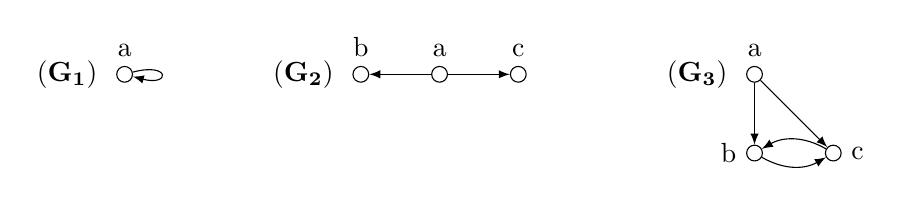
\begin{tikzpicture}
      [
      point/.style={circle,draw,inner sep=0pt,minimum size=2mm},
      collection/.style={thick,rectangle,draw,inner sep=0pt,minimum height=14mm, minimum width= 9mm}
      ]
      \node (label) at (0,1) [label=left:$(\mathbf{G_1})\;$] {};
      \node (0) at (0,1) [point,label=above:a] {};
      \draw [-latex, loop right] (0) to (0);

      \node (label) at (3,1) [label=left:$(\mathbf{G_2})\;$] {};
      \node (0) at (4,1) [point,label=above:a] {};
      \node (1) at (3,1) [point,label=above:b] {};
      \node (2) at (5,1) [point,label=above:c] {};
      \draw [-latex] (0) to (1);
      \draw [-latex] (0) to (2);

      \node (label) at (8,1) [label=left:$(\mathbf{G_3})\;$] {};
      \node (0) at (8,1) [point,label=above:a] {};
      \node (1) at (8,0) [point,label=left:b] {};
      \node (2) at (9,0) [point,label=right:c] {};
      \draw [-latex] (0) to (2);
      \draw [-latex] (0) to (1);
      \draw [-latex, bend right] (1) to (2);
      \draw [-latex, bend right] (2) to (1);
    \end{tikzpicture}
  \]
  Using the graphs from above, we get the following theories using $\mathcal{T}$:
  \begin{align}
    \mathcal{T}(\mathbf{G_1}) &= \big \{ a \leftrightarrow \neg a \big \} \\
    \mathcal{T}(\mathbf{G_2}) &= \big \{ a \leftrightarrow (\neg b \wedge \neg c), b, c \big \}\\
    \mathcal{T}(\mathbf{G_3}) &= \big \{ a \leftrightarrow (\neg b \wedge \neg c), b \leftrightarrow \neg c, c \leftrightarrow \neg b \big \}
  \end{align}

\end{example}
The fact that $sol(\mathbf{G}) = mod(\mathcal{T}(G))$ is shown in \cite{apal-digraph}.
Allthough not proving it, we can observe that $\mathbf{G_1}$ has no solution, just like its corresponding theory $\mathcal{T}(\mathbf{G_1})$ has no models.
$\mathbf{G_2}$ has one solution, where one assigns $a=0, b=1, c=1$.
This assignment also works as a model for $\mathcal{T}(\mathbf{G_2})$.
In $\mathbf{G_3}$, we get two solutions, both with $a$ assigned to 0, but with 0 and 1 distributed on $b$ and $c$.
These are also the only two models of $\mathcal{T}(\mathbf{G_3})$.

Conversely, given any discourse theory $T$ (in fact, this will work given any PL theory, since we can translate CNF to GNF), we can derive the corresponding graph $\mathcal{G}(T)$ in the following way:
All variables in the theory are vertices, and for each formula $x \leftrightarrow \bigwedge_{y \in I_x} y$ make a directed edge $\langle x,y \rangle$ for each $y \in I_x$.\\

\begin{example}
  \begin{align}
    ( a \lar \neg a'), (a' \lar \neg a), (b \lar \neg b'), (b' \lar \neg b), (y_1 \lar (\neg a \wedge \neg b \wedge \neg y_1))
  \end{align}
  Using $\mathcal{G}$ on the above GNF theory gives us the following graph:
  \[
    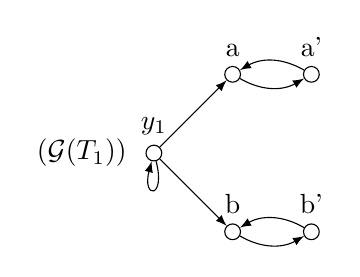
\begin{tikzpicture}
      [
      point/.style={circle,draw,inner sep=0pt,minimum size=2mm},
      collection/.style={thick,rectangle,draw,inner sep=0pt,minimum height=14mm, minimum width= 9mm}
      ]
      \node (label) at (5,1) [label=left:$(\mathcal{G}(T_1))\;$] {};
      \node (0) at (5,1) [point,label=above:$y_1$] {};
      \node (1) at (6,0) [point,label=above:b] {};
      \node (2) at (7,0) [point,label=above:b'] {};
      \node (3) at (6,2) [point,label=above:a] {};
      \node (4) at (7,2) [point,label=above:a'] {};
      \draw [-latex, loop below] (0) to (0);
      \draw [-latex] (0) to (1);
      \draw [-latex, bend right] (1) to (2);
      \draw [-latex, bend right] (2) to (1);
      \draw [-latex] (0) to (3);
      \draw [-latex, bend right] (3) to (4);
      \draw [-latex, bend right] (4) to (3);
    \end{tikzpicture}
  \]
\end{example}
Again, will we not be proving the correspondence, but notice that $T_1$ has one model satisfying it, where $a = 0$.
$\mathcal{G}(T_1)$ also has one solution, namely where $a = 0, a' = 1, y_1 = 0$.
$T_2$ has three solutions, where either $a$, $b$ or both are assigned $1$.
This reflects onto the graph since $y_1$ has to be assigned $0$, thus forcing $a$ or $b$ to be assigned $1$.
The fact that $\mathcal{G}$ gives us the correspondence we are looking for is shown in \cite{apal-digraph}.

This equivalence connects the fields of logic with the fields of graph theory:
With the problem of solutions in the graph being equivalent with SAT, we get our final equivalence between kernels in the graph and models of the theory.
A graph has a kernel if and only if its corresponding discourse is consistent (non-paradoxical).
A theory is paradoxical if and only if its corresponding graph has no kernels.
Because of this tight link, we will often refer to graphs without kernels as paradoxical graphs.

The applicability of kernels should by now be obvious.
In the next section we will review some of the various findings within Kernel Theory, and especially the findings related to infinitary graphs.

	% !TEX root= ../main.tex
\section{Results in Kernel Theory}
\label{sec:Results in Kernel Theory}
The end goal within Kernel Theory is ultimately to develop an easy way of answering the question ``Does this digraph have a kernel?'' no matter the graph, and no matter the answer.
As of today, we are not quite there, but a lot of work has been put into trying to identify special circumstances under which one is guaranteed to have (or guaranteed to not have) a kernel in the given graph.
One of the results is the Richardson's Theorem\cite{am-richardson}, worked out by Moses Richardson in 1953:\\

\begin{theorem}
  If D is a finitary\footnote{In a finitary graph, every vertex has a finite number of out-neighbors; the graph has finite branching.} digraph without odd cycles, then D has a kernel.
\end{theorem}

Intuitively, one might be tempted to believe that \textit{all} digraphs without odd cycles have kernels, but this is not the case.
Until now, our paradoxes have always been statements that -- directly or indirectly -- have been referring back to themselves (giving cycles in the graph) and thus causing a logical conflict, and it is hard to imagine any other way to construct paradoxical statements.
The following construction will however reveal our lack of imagination.

The \textit{Yablo Graph}\cite{analysis-yablo} is an example of an acyclic graph with no kernel.
It is constructed with an infinite set of vertices $\{ x_i | i \in \mathbb{N} \}$ and a set of edges $N$ such that $\langle x_i, x_j \rangle \in N$ iff $i < j$.
\[
  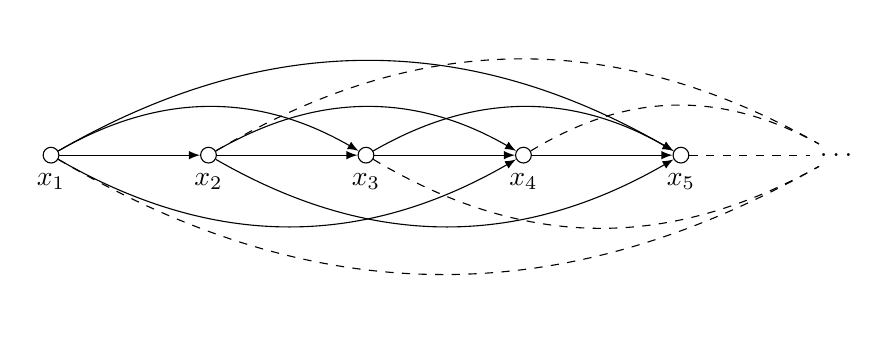
\begin{tikzpicture}
    [
    point/.style={circle,draw,inner sep=0pt,minimum size=2mm},
    collection/.style={thick,rectangle,draw,inner sep=0pt,minimum height=14mm, minimum width= 9mm}
    ]
    \node (1) at (0,1) [point,label=below:$x_1$] {};
    \node (2) at (2,1) [point,label=below:$x_2$] {};
    \node (3) at (4,1) [point,label=below:$x_3$] {};
    \node (4) at (6,1) [point,label=below:$x_4$] {};
    \node (5) at (8,1) [point,label=below:$x_5$] {};
    \node (6) at (10,1) [] {$\dots$};
    \draw [-latex] (1) to (2);
    \draw [-latex] (2) to (3);
    \draw [-latex] (3) to (4);
    \draw [-latex] (4) to (5);
    \draw [dashed] (5) to (6);
    \draw [-latex, bend left] (1) to (3);
    \draw [-latex, bend left] (2) to (4);
    \draw [-latex, bend left] (3) to (5);
    \draw [dashed, bend left] (4) to (6);
    \draw [-latex, bend right] (1) to (4);
    \draw [-latex, bend right] (2) to (5);
    \draw [dashed, bend right] (3) to (6);
    \draw [-latex, bend left] (1) to (5);
    \draw [dashed, bend left] (2) to (6);
    \draw [dashed, bend right] (1) to (6);
  \end{tikzpicture}
\]
Since there exist no two numbers $x,y \in \mathbb{N}$ such that $x < y$ and $y < x$, we get that the Yablo graph indeed is acyclic\todo{This is a bit over-simplified}.
Furthermore, since any natural number has infinitely many numbers strictly larger than it, we get that all the vertices are infinitely branching, making the Yablo graph infinitary (non-finitary).

The discourse represented by the Yablo graph would -- informally -- be the situation with an infinite number of statements, all saying ``Every statement after this statement is false''.

We will later show formally that the Yablo-graph is indeed without a kernel, but for now the following explanation will do.

Let us assume that the Yablo-graph \textit{has} a kernel and that the vertex $x_a$ is in it.
Then all the vertices to the right of $x_a$ are necessarily outside of the kernel, including $x_{a+1}$.
But if $x_{a+1}$ is outside of the kernel, it has to point to a vertex on the inside.
This is now impossible, since the out-neighborhood of $x_{a+1}$ is a subset of the out-neighborhood of $x_a$.
Since $x_a$ was chosen without any restrictions, no vertex can be inside the kernel, making it empty.
This is oviously not possible, so the Yablo-graph is without a kernel.

One thing should be mentioned at this point; neither odd cycles nor infinitely branching vertices \textit{entail} that their respective graphs are paradoxical.
The two following graphs illustrate this point:
\begin{align}
  \begin{aligned}
    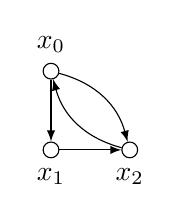
\begin{tikzpicture}
      [
      point/.style={circle,draw,inner sep=0pt,minimum size=2mm},
      collection/.style={thick,rectangle,draw,inner sep=0pt,minimum height=14mm, minimum width= 9mm}
      ]
      \node (0) at (0,1) [point,label=above:$x_0$] {};
      \node (1) at (0,0) [point,label=below:$x_1$] {};
      \node (2) at (1,0) [point,label=below:$x_2$] {};
      \draw [-latex] (0) to (1);
      \draw [-latex] (1) to (2);
      \draw [-latex, bend left] (2) to (0);
      \draw [-latex, bend left] (0) to (2);
    \end{tikzpicture}
  \end{aligned}
\end{align}
The above graph contains an odd cycle, but the singleton set $\{x_2\}$ is a kernel.
\begin{figure}[!h]
  \centering
  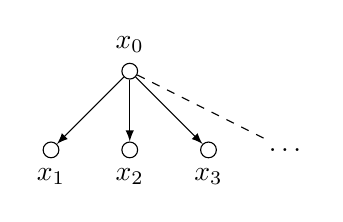
\begin{tikzpicture}
    [
    point/.style={circle,draw,inner sep=0pt,minimum size=2mm},
    collection/.style={thick,rectangle,draw,inner sep=0pt,minimum height=14mm, minimum width= 9mm}
    ]
    \node (0) at (1,2) [point,label=above:$x_0$] {};
    \node (1) at (0,1) [point,label=below:$x_1$] {};
    \node (2) at (1,1) [point,label=below:$x_2$] {};
    \node (3) at (2,1) [point,label=below:$x_3$] {};
    \node (4) at (3,1) [] {$\dots$};
    \draw [-latex] (0) to (1);
    \draw [-latex] (0) to (2);
    \draw [-latex] (0) to (3);
    \draw [dashed] (0) to (4);
  \end{tikzpicture}
  \caption{}
  \label{infinitary_with_kernel}
\end{figure}

The above graph has an infinitely branching vertex $x_0$, but the infinite set $\{x_i \;|\; x > 0\}$ is a kernel.

It is shown in \cite{apal-digraph} that every digraph (with at least one edge) can be transformed into a infinitary dag\footnote{Directed acyclic graph} such that $\alpha$ is a solution to the created dag if and only if it is a solution to the original digraph.
This means that for any finitary graph that is paradoxical by the virtue of having an odd cycle, there is an infinitary, \textit{acyclic} digraph that is also paradoxical.
So, if one is trying to find ways to identify paradoxical graphs, one does only need to look at dags.

This result will be of great importance to us, enabling us to narrow our search space when looking for paradoxes.

	% !TEX root= ../main.tex
\externaldocument{kernelthoery}
\section{Recognizing dags without kernels}
\label{sec:Recognizing dags without kernels}
Knowing that any graph can be translated to an equisatisfiable dag, the challenge is now to find sufficient conditions for dags to have kernels, even weaker than the one proved by Richardson (the fact that any finitary dag has a kernel is a direct consequence of Richardson's Theorem).

Michał Walicki has proposed the following thesis:
\begin{quote}
  ``If a dag has no kernel then it has a ray with infinitely many vertices dominating it.''
\end{quote}
Some terminology (given a graph $\mathbf{G} = \langle G,N \rangle$):
A \textit{ray} is an semi-infinite path, i.e. an infintie sequence $(x_1, x_2, \dots)$ of distinct vertices of $G$ such that $(x_i,x_{i+1}) \in N$ for each $i$.

A vertex $x_0$ \textit{dominates} a set of vertices $Y \subseteq G$ if there exists an infinite number of disjoint paths from $x_0$ to distinct vertices of $Y$.

The contrapositive of Walicki's thesis suggests a weaker condition for a kernel, since a dag having a ray with infinitely many vertices dominating it implies that the dag is infinitary.

	% !TEX root= ../main.tex
\externaldocument{discoursegraphs}
\externaldocument{kerneltheory}
\section{Resolving GNF-theories}
\label{sec:Resolving GNF-theories}
In this section, we present an inference system introduced by Walicki in \cite{michal-completeness} which handles clausal theories induced from GNF-theories.

Recall that a theory written in GNF has formulae of the following form:
\begin{align}
  x \lar \bigwedge_{i \in I_x} \neg y_i
\end{align}
Using simple operations only, one can manipulate these formulae into an equivalent set of clauses.
We start by writing the above bi-implication as two implications:
\begin{align}
  x \rightarrow \bigwedge_{i \in I_x} \neg y_i \quad\quad \text{and} \quad\quad x \leftarrow \bigwedge_{i \in I_x} \neg y_i
\end{align}
The first implication can be rewritten in the following way:
\begin{align}
  x \rightarrow \bigwedge_{i \in I_x} \neg y_i
  \quad\Leftrightarrow\quad \neg x \vee \bigwedge_{i \in I_x} \neg y_i
  \quad\Leftrightarrow\quad \bigwedge_{i \in I_x} (\neg x \vee \neg y_i)
  \quad\Leftrightarrow\quad \bigwedge_{i \in I_x} \neg (x \wedge y_i)
\end{align}
The second implication can be rewritten in the following way:
\begin{align}
  x \leftarrow \bigwedge_{i \in I_x} \neg y_i
  \quad\Leftrightarrow\quad x \vee \neg \left( \bigwedge_{i \in I_x} \neg y_i \right)
  \quad\Leftrightarrow\quad x \vee \bigvee_{i \in I_x} y_i
\end{align}
By splitting the conjunction from the first implication up into individual clauses, we get the following two kinds of clauses for every variable $x$ in the GNF theory:
\begin{align}
  \text{OR-clause:}&\quad x \vee \bigvee_{i \in I_x} y_i\\
  \text{NAND-clauses:}&\quad \neg (x \wedge y_i)\text{, for every }i \in I_x
\end{align}
We will treat both the OR-clauses and the NAND-clauses as sets of atoms, denoting NAND-clauses $\neg (x \wedge y)$ as $\overline{xy}$ and OR-clauses $x \vee y_1 \vee y_2 \vee y_3$ as $xy_1y_2y_3$.
This enables us to state things like $\overline{xy} \subset \overline{xyz}$.
A theory will -- as expected -- be a set of OR- and NAND-clauses.

If we interpret the initial GNF-theory as a graph $\mathbf{G}=\langle G,N\rangle$, for every vertex $x \in G$, there will be one OR-clause $\{ x \} \cup N(x)$ and for every edge $\langle x,y \rangle \in N$ there will be a NAND-clause $\overline{xy}$.
The graphs from Example~\ref{ex:3graphs} will have the following clausal theories:
\begin{align}
  \mathcal{T}(\mathbf{G_1}) &= \{ a, \ol{a} \}\\
  \mathcal{T}(\mathbf{G_2}) &= \{ abc, b, c, \ol{ab}, \ol{ac} \}\\
  \mathcal{T}(\mathbf{G_3}) &= \{ abc, bc, \ol{ab}, \ol{bc} \}
\end{align}
Further notation: $A\subseteq G$ denotes an OR-clause while $\ol{A} \subseteq G$ denotes a NAND-clause.
Given a graph $\mathbf{G}=\langle G,N\rangle$, we denote the set of all NAND-clauses induced from the graph as NAND and all induced OR-clauses as OR.
The combined set $\Gamma = NAND + OR$ will be our initial clauses in the inference system.
\subsection{The inference system}
\label{sub:The inference system}
We consider the following inference system, but we will focus mainly on proofs using the Axioms together with the (Rneg) rule.
\begin{align}
  \text{(Ax)} &\quad \Gamma \vdash C, \quad \text{for } C \in \Gamma\\
  \text{(Rneg)} &\quad \frac{ \{ \Gamma \vdash \ol{a_iA_i} \; |\; i \in I \} \quad \Gamma \vdash \{ a_i \; |\; i \in I \} }{ \Gamma \vdash \ol{\bigcup_{i \in I} A_i} }\\
  \text{(Rpos)} &\quad \frac{ \Gamma \vdash A \quad \{\Gamma \vdash B_iK_i \; |\; i \in I \} \quad \{ \Gamma \vdash \ol{a_ik} \; |\; i \in I, k \in K_i \} }{ \Gamma \vdash (A \setminus \{ a_i \; |\; i \in I \} ) \cup \bigcup_{i \in I} B_i }
\end{align}
(Rneg) is creating NAND-clauses from NAND-clauses using OR as a side-condition.
(Rpos) is creating OR-clauses from OR-clauses using NAND as a side-condition.
In (Rneg), $\ol{a_iA_i}$ denotes the NAND $\ol{\{ a_i \} \cup A_i}$ with a potentially empty $A_i$.

The premise of the (Rneg) rule is a set of $I$ NAND-clauses together with one OR-clause with $I$ elements such that each atom $a_i$ in the OR-clause is contained within a NAND-clause, and such that each NAND-clause contains an atom from the OR-clause.
The correspondence between the NAND-clauses and the elements of the OR-clause should in other words be bijective.
The conclusion is the union of all the NAND-clauses without their corresponding atom from the OR-clause.

Here are some examples of incorrect applications of the (Rneg)-rules, followed by some correct applications:
\begin{align}
  (1)\;\;\frac{\ol{ax}\quad\ol{by}\quad\ol{cz}}{\ol{xyz}}abx\quad\quad
  (3)\;\;\frac{\ol{ax}\quad\ol{by}}{\ol{xy}}abx\quad\quad
  (2)\;\;\frac{\ol{ax}\quad\ol{by}\quad\ol{bz}}{\ol{xyz}}abx
\end{align}
(1) is incorrect because the NAND $\ol{cz}$ contains no atoms from the OR $abx$.
(2) is incorrect because the number of NAND-clauses does not match the length of the OR-clause.
(3) is incorrect because there exist no bijective correspondence of the type described above.
\begin{align}
  (4)\;\;\frac{\ol{ax}\quad\ol{by}\quad\ol{cz}}{\ol{xyz}}abc\quad\quad
  (5)\;\;\frac{\ol{ax}\quad\ol{b}}{\ol{x}}ab\quad\quad
  (6)\;\;\frac{\ol{ax}\quad\ol{by}\quad\ol{xyz}}{\ol{xyz}}abx
\end{align}
The three above applications are all correct, since all the atoms in each OR-clause get matched to exactly one NAND-clause in such a way that no NAND-clause stays unmatched.

We set no restrictions on the number and cardinality of our clauses, meaning that there might be an infinite number of clauses, and both the OR-clauses and the NAND-clauses might be either finite or infinite in size.
Note that an infinite graph gives infinitely many NAND-clauses, while an infinitary graph also gives us infinitely long OR-clauses.

We study the refutation system that arises from the Axioms and the (Rneg)-rule, calling it Neg.
It is shown in \cite{michal-completeness} that Neg is sound and refutationally complete for theories with only a countable number of OR-clauses.
Soundness gives us that proving $\ol{C}$ for any $C \subseteq G$ implies that the vertices in $C$ cannot all be assigned 1 in the graph model.
Refutational completeness gives us that whenever a graph/theory is inconsistent, we are able to prove $\varnothing$ in Neg.

Note that Neg is not complete.
The following inconsistent graph exemplifies this:\par
\begin{figure}[!h]
  \centering
  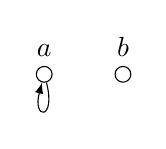
\begin{tikzpicture}
    [
    point/.style={circle,draw,inner sep=0pt,minimum size=2mm}
    ]
    \node (1) at (0,0) [point, label=above:$a$] {};
    \node (2) at (1,0) [point, label=above:$b$] {};
    \draw [-latex, loop below] (1) to (1);
  \end{tikzpicture}
  \caption{}
  \label{fig:neg_not_complete}
\end{figure}
Bacause of the loop on vertex $a$, the graph has no solutions.
We therefore have $\vDash \ol{b}$, but we are unable to prove $\ol{b}$ in Neg.
\subsection{Inconsistency of the Yablo-graph}
\label{sub:Inconsistency of the Yablo-graph}
The inconsistency of the Yablo-graph is easily proven using Neg only.
Since every vertex $x_i$ (using the notation from Figure~\ref{fig:yablo-graph}) has an edge to each vertex $x_j$ where $j > i$, we get that every pair of distinct vertices is connected by an edge.
This means that our set of axioms from the Yablo-graph looks like this:
\begin{align}
  \text{NAND} = \{ \ol{x_ix_j} \; |\; i < j\}
  \quad\quad\quad
  \text{OR} = \{ x_ix_{i+1}x_{i+2}\dots \; |\; i \in \mathbb{N}\}
\end{align}
For any vertex $x_i$ from the Yablo-graph, we are now able to prove $\ol{x_i}$ in the following way:
\begin{prooftree*}
  \Hypo{\ol{x_ix_{i+1}}}
  \Hypo{\ol{x_ix_{i+2}}}
  \Hypo{\ol{x_ix_{i+3}}}
  \Hypo{\dots}
  \Infer4[$x_ix_{i+1}x_{i+2}\dots$]{\ol{x_i}}
\end{prooftree*}
Proving $\varnothing$ is now simple:
\begin{prooftree*}
  \Hypo{\dots}
  \Infer1{\ol{x_1}}
  \Hypo{\dots}
  \Infer1{\ol{x_2}}
  \Hypo{\dots}
  \Infer1{\ol{x_3}}
  \Hypo{\dots}
  \Infer4[$x_1x_2x_3\dots$]{\varnothing}
\end{prooftree*}
A less trivial inconsistency proof is the one on the \textit{Stretched Yablo-graph}.
This proof can be found in the appendix together with the definition of Stretched Yablo.

It is worth mentioning that even though our focus has been -- and will be -- on theories originating from graphs, the results on soundness and completeness holds for any theory consisting of a set of NANDs and a set of ORs.

An example of this is the pigeonhole problem which easily can be represented as a set of NAND- and OR-clauses, but does not directly correspond to a graph (it can of course be translated to a graph theory, like any other propositional theory).
Proofs in Neg of pigeonhole problems of different size are to be found in the appendix\todo{some reference system needed}.

	% !TEX root= ../main.tex
\section{Thesis overview}
\label{sec:Thesis overview}
The soundness and refutational completeness of Neg makes it a potentially great tool in the overarching endeavor of weakening the conditions for kernels in graphs.
We know that for any graph $G$, $\varnothing$ can be proven in Neg based on $G$ if and only if $G$ is without a kernel.

Suppose that any inconsistency can be proven using only NAND-clauses of length at most 2, and that all NAND-clauses of length 2 corresponds to vertices related in a certain way in the graph.
This would in combination give us a condition for kernels, namely the absence of such specifically related vertices.
With this in mind, the thesis will set out to do two things:

(1) Define a graph structural relation such that two vertices $a,b$ in a graph $G$ are related if and only if $G \vdash \ol{ab}$.

This will be covered in Chapter 2 where we will be looking at increasingly general graph structures that ensures the provability of certain NAND-clauses, ultimately attempting to reach a structure general enough so that the provability of a NAND-clause entails the existence of that structure.

(2) Explore whether Neg is still refutationally complete when restricted to using NAND-clauses of length 1 or 2 only.

It will be shown in Chapter 3 that this is \textit{not} possible.
The chapter will present graphs where certain NAND-clauses are provable in general, but not under the restrictions mentioned.
This will then be used to show that the restrictions makes Neg unable to prove inconsistencies in certain graphs.

	\chapter{NAND-clauses in graphs}
	\label{chap:NAND-clauses in graphs}
	% !TEX root= ../main.tex
In this chapter we will motivate and conduct the search for graph structural equivalents of unary and binary NAND-clauses proven in Neg.
An actual graph structure corresponding to the NAND-clauses will not be presented, but we will show some graph structures implying certain provable NAND-clauses.
\begin{definition}
  A clause is \textit{unary} if it contains only one atom.
  A clause is \textit{binary} if it consists of one or two atoms.\todo{should both lengths be included?}
\end{definition}

	% !TEX root= ../main.tex
\section{Motivation}
\label{sec:Motivation}
Since our proof system, Neg, has only one rule, the last step of any inconsistency proof will always look the same:\par
\begin{figure}[!h]
  \centering
  \begin{prooftree*}
    \Hypo{\ol{x_1}}
    \Hypo{\ol{x_2}}
    \Hypo{\ol{x_3}}
    \Hypo{\dots}
    \Infer4[$x_1x_2x_3\dots$]{\varnothing}
  \end{prooftree*}
  \caption{}
  \label{fig:proof_unary_nand}
\end{figure}
The premise will always consist of a collection of NAND-clauses, each of length 1, together with an OR-clause equal to the union of all the NAND-clauses.
It is easy to see that none of the NAND-clauses can be larger than unary, since that would result in a non-empty NAND-clause in the conclusion.
The OR-clause has to equal the union of the NAND-clauses simply by definition of the (RNeg)-rule.

This fact was also observed and formalized by Walicki\cite{michal-completeness}:
\begin{align}
  \Gamma \vdash \{\} \Leftrightarrow \exists K \in \text{OR}: (\forall  k \in K: \Gamma \vdash \ol{k})
\end{align}
We know from the definition that any OR-clause used in the proof system corresponds to a single vertex with its successors in the graph.
We do however not know what the NAND-clauses of length 1 might correspond to.
Knowing this would, by soundness and completeness of Neg, give us the graph structure needed for a kernel not to exist.
\todo{Currently brushing over the restrictions set to the proofs of completeness and soundness. Will fix this later.}

The only thing we \textit{do} know about unary NAND-clauses is that they correspond to vertices that are assigned 0 in all models of the graph.
We get this from soundness of Neg.
This is however not the graph structural property we are ultimately looking for, but we can at least say that we have reduced the question ``What does an inconsistent graph look like?'' to the question ``What does a provably false vertex look like?''.

So what does a unary NAND-clause proven in Neg correspond to in the graph?
Similarly to a proof of $\varnothing$, there is really just one way to prove a unary NAND-clause:\par
\begin{figure}[!h]
  \centering
  \begin{prooftree*}
    \Hypo{\ol{xy_1}}
    \Hypo{\ol{xy_2}}
    \Hypo{\dots}
    \Hypo{\ol{y_n}}
    \Hypo{\ol{y_{n+1}}}
    \Hypo{\dots}
    \Infer6[$y_1y_2\dots y_ny_{n+1}\dots$]{\ol{x}}
  \end{prooftree*}
  \caption{}
  \label{fig:proof_unary_nand}
\end{figure}
Any derivation of a unary NAND-clause $\ol{x}$ must end with a rule application using $K \in \text{OR}$ where for each $k \in K$, there is a NAND-clause in the premise that is either unary, $\ol{k}$ or binary, $\ol{xk}$.
In addition, we require the premise to contain at least one binary NAND-clause, in order to actually be able to conclude with $\ol x$ and not $\varnothing$.

We formalize this observation in the following way:
\begin{align}
  \Gamma \vdash \ol{x} \Leftrightarrow \exists K \in \text{OR}:
  \left ( \begin{tabular}{l}
  $\exists k \in K: G \vdash \ol{kx} \; \wedge$\\
  $\forall k \in K: G \vdash \ol{kx} \vee G \vdash \ol{k}$
  \end{tabular} \right )
\end{align}
Just as we reduced the problem of inconsistency to the problem of unary NAND-clauses, we are able to reduce the problem further to binary NAND-clauses.
We could even continue the reduction further to ternary clauses, quaternary clauses and so on, but without a change of strategy at some point, this seems pointless.

Our current reduction lets us ask how two vertices $x,y$ are \textit{connected} in the graph when their binary NAND $\ol{xy}$ is proven in Neg.
Observe that we have parts of this correspondence down already, with our axioms being all binary.
Vertices directly connected by an edge must therefore be a part of the corresponding graph structure.
%Finding some graph structural relation that corresponds to binary NAND-clauses might also give us some knowledge about a potential standard form of binary-NAND-proofs.\todo{does this make sense?}

Let $R(a,b)$ denote the existence of some graph structure $R$ between the vertices $a$ and $b$ in some graph $G$; our correspondence can now be formally defined as follows:
\begin{align}
  (1) \quad R(a,b) \quad \Rightarrow \quad G \vdash \ol{ab}\\
  (2) \quad R(a,b) \quad \Leftarrow \quad G \vdash \ol{ab}
\end{align}
The two implications will be referred to as \textit{implication (1)} and \textit{implication (2)}, respectively.

Suppose we manage to find a structure $R$ that satisfied both above implications.
The following equation tells us how that would directly give us a predicate deciding whether or not the graph has a kernel.\todo{This should be rewritten.}
\begin{align}
  &Sol(G) = \varnothing\\
  \Leftrightarrow\; &G \vdash \varnothing\\
  \overset{2.1}{\Leftrightarrow}\;&\exists K \in \text{OR}: (\forall  k \in K: G \vdash \ol{k})\\
  \overset{2.2}{\Leftrightarrow}\;&\exists K \in \text{OR}: (\forall  k \in K: ( \exists L \in \text{OR}:
  \left ( \begin{tabular}{l}
  $\exists l \in L: G \vdash \ol{lk} \; \wedge$\\
  $\forall l \in L: G \vdash \ol{lk} \vee G \vdash \ol{l}$
  \end{tabular} \right ) ) )\\
  \overset{2.3}{\underset{2.4}{\Leftrightarrow}}\;&\exists K \in \text{OR}: (\forall  k \in K: ( \exists L \in \text{OR}:
  \left ( \begin{tabular}{l}
  $\exists l \in L: G \vdash R(l,k) \; \wedge$\\
  $\forall l \in L: G \vdash R(l,k) \vee G \vdash R(l,l)$
  \end{tabular} \right ) ) )
\end{align}
The next sections will present various graph structures, each satisfying implication (1).
Each presented structure will be a generalization of the previous one, ultimately aiming to find a structure general enough to satisfy both implication (1) and implication (2).
Such a structure would be the true graph structural equivalent of a binary NAND provable in Neg.
We did however not manage to find such a graph structure in this thesis.

For each structure presented, implication (1) will be shown, followed by an example disproving implication (2).
The counterexamples will be graphs with the presented structure absent, but where the corresponding NAND-clause is still provable.

Because of soundness of Neg, if two vertices correspond to a provable binary NAND in Neg, for any kernel $K$ in that graph, at least one of the two vertices is outside $K$.
The contrapositive of this observation being that for a graph $G$, if there exists a kernel $K \subseteq G$ such that two vertices, $x_1$ and $x_2$ are both in $K$, then $\ol{x_1x_2}$ is not provable from $G$.
This fact will be used when arguing why some graph structures are \textit{not} satisfying implication (1).

	% !TEX root= ../main.tex
\section{Odd paths}
\label{sec:Odd paths}
Given two vertices $x_1$ and $x_2$ in a graph $G$, if we in Neg are able to prove $\ol{x_1x_2}$ from the axioms we get from $G$, we say that $x_1$ and $x_2$ are \textit{vel-connected}.
This section will try to answer the question ``what kind of graph structures imply that certain vertices are vel-connected?''.

Because of soundness of Neg, we get that if two vertices are vel-connected in a graph, for each kernel $K$ in that graph, at least one of the two vertices are outside $K$.
The counterpositive being that for a graph $G$, if there exists a kernel $K \subseteq G$ such that two vertices, $x_1$ and $x_2$ are both in $K$, then $x_1$ and $x_2$ cannot be vel-connected in $G$.
This fact will be used in argumenting for why some graph structures are not giving us vel-connected vertices.

We already know that whenever two vertices are connected by an edge, their binary NAND is trivially provable in Neg, since it will be a part of the axioms.

We illustrate this case with the figure below, where dashed lines represent possible out-edges to irrelevant parts of the graph.
If a vertex has no dashed edges, it means that we disallow any additional edges out from this vertex.
\[
  \begin{tikzpicture}
    [
    point/.style={circle,draw,inner sep=0pt,minimum size=2mm},
    ]
    \node (1) at (1,1) [point] {};
    \node (2) at (2,1) [point] {};
    \draw [-latex] (1) to (2);

    \node (e1) [above left=4mm and 6mm of 1]  {};
    \node (e2) [left=8mm of 1] {};
    \node (e3) [below left=4mm and 6mm of 1] {};
    \node (e4) [above right=4mm and 6mm of 2] {};
    \node (e5) [right=8mm of 2] {};
    \node (e6) [below right=4mm and 6mm of 2] {};
    \draw [dashed] (e1) to (1);
    \draw [dashed] (e2) to (1);
    \draw [dashed] (e3) to (1);
    \draw [dashed] (e4) to (2);
    \draw [dashed] (e5) to (2);
    \draw [dashed] (e6) to (2);
  \end{tikzpicture}
\]
The basic example above tells us that two vertices are vel-connected when one is the successor of the other.
It is however easy to find a case examplifying how the implication does not hold in the opposite direction.
\[
  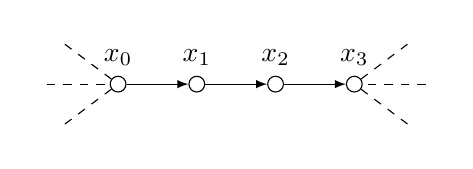
\begin{tikzpicture}
    [
    point/.style={circle,draw,inner sep=0pt,minimum size=2mm},
    ]
    \node (1) at (0,1) [point,label=above:$x_0$] {};
    \node (2) at (1,1) [point,label=above:$x_1$] {};
    \node (3) at (2,1) [point,label=above:$x_2$] {};
    \node (4) at (3,1) [point,label=above:$x_3$] {};
    \draw [-latex] (1) to (2);
    \draw [-latex] (2) to (3);
    \draw [-latex] (3) to (4);

    \node (e1) [above left=4mm and 6mm of 1]  {};
    \node (e2) [left=8mm of 1] {};
    \node (e3) [below left=4mm and 6mm of 1] {};
    \node (e4) [above right=4mm and 6mm of 4] {};
    \node (e5) [right=8mm of 4] {};
    \node (e6) [below right=4mm and 6mm of 4] {};
    \draw [dashed] (e1) to (1);
    \draw [dashed] (e2) to (1);
    \draw [dashed] (e3) to (1);
    \draw [dashed] (e4) to (4);
    \draw [dashed] (e5) to (4);
    \draw [dashed] (e6) to (4);
  \end{tikzpicture}
\]
The above graph provides us the following axioms:
$NAND = \{\ol{x_0x_1},\ol{x_1x_2},\ol{x_2x_3}\}$, $OR = \{x_0x_1,x_1x_2,x_2x_3\}$.
From these axioms, we can now, despite the fact that the vertices $x_0$ and $x_3$ are not connected by an edge, easily prove the NAND-clause $\ol{x_1x_4}$:.

\begin{prooftree*}
  \Hypo{\ol{x_0x_1}}
  \Hypo{\ol{x_2x_3}}
  \Infer[left label=$x_1x_2$]2{\ol{x_0x_3}}
\end{prooftree*}

Intuitively, one can imagine that the proof above is connecting two NAND-clauses using an OR-clause, resulting in a new binary NAND-clause containing vertices that are weaklier connected than the ones we started with.
This can be done repeatedly, resulting in the ability to prove binary NAND-clauses from vertices that are connected by arbitrarily long paths of the kind above.

Consider the following graph:
\[
  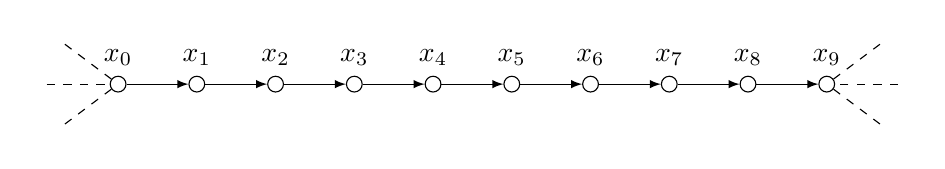
\begin{tikzpicture}
    [
    point/.style={circle,draw,inner sep=0pt,minimum size=2mm},
    ]
    \node (1) at (0,1) [point,label=above:$x_0$] {};
    \node (2) at (1,1) [point,label=above:$x_1$] {};
    \node (3) at (2,1) [point,label=above:$x_2$] {};
    \node (4) at (3,1) [point,label=above:$x_3$] {};
    \node (5) at (4,1) [point,label=above:$x_4$] {};
    \node (6) at (5,1) [point,label=above:$x_5$] {};
    \node (7) at (6,1) [point,label=above:$x_6$] {};
    \node (8) at (7,1) [point,label=above:$x_7$] {};
    \node (9) at (8,1) [point,label=above:$x_8$] {};
    \node (10) at (9,1) [point,label=above:$x_9$] {};
    \draw [-latex] (1) to (2);
    \draw [-latex] (2) to (3);
    \draw [-latex] (3) to (4);
    \draw [-latex] (4) to (5);
    \draw [-latex] (5) to (6);
    \draw [-latex] (6) to (7);
    \draw [-latex] (7) to (8);
    \draw [-latex] (8) to (9);
    \draw [-latex] (9) to (10);

    \node (e1) [above left=4mm and 6mm of 1]  {};
    \node (e2) [left=8mm of 1] {};
    \node (e3) [below left=4mm and 6mm of 1] {};
    \node (e4) [above right=4mm and 6mm of 10] {};
    \node (e5) [right=8mm of 10] {};
    \node (e6) [below right=4mm and 6mm of 10] {};
    \draw [dashed] (e1) to (1);
    \draw [dashed] (e2) to (1);
    \draw [dashed] (e3) to (1);
    \draw [dashed] (e4) to (10);
    \draw [dashed] (e5) to (10);
    \draw [dashed] (e6) to (10);
  \end{tikzpicture}
\]

$\ol{x_0x_9}$ can now be proven in Neg in the following way:
\begin{prooftree*}
  \Hypo{\ol{x_0x_1}}
  \Hypo{\ol{x_2x_3}}
  \Infer[left label=$x_1x_2$]2{\ol{x_0x_3}}
  \Hypo{\ol{x_4x_5}}
  \Infer[left label=$x_4x_5$]2{\ol{x_0x_5}}
  \Hypo{\ol{x_6x_7}}
  \Infer[left label=$x_6x_7$]2{\ol{x_0x_7}}
  \Hypo{\ol{x_8x_9}}
  \Infer[left label=$x_8x_9$]2{\ol{x_0x_9}}
\end{prooftree*}

Observe that the above proof is also proving $\ol{x_0x_3}$, $\ol{x_0x_5}$ and $\ol{x_0x_7}$ along the way, all in which contain vertices connected by paths of \textit{odd} length.
This is an important point.
NAND-clauses containing vertices connected only by paths of \textit{even} length cannot be proven in the same manner as above.
Usually, such NAND-clauses cannot be proven at all.

It is also worth noting that all the paths so far have been stripped for any branching, keeping the OR-clauses binary in length.
We will call these kinds of paths \textit{fully trimmed paths}, and formally define them as paths where for each contained vertex $x$ and its successor in the path $y$, we have that $N(x) = \{y\}$.

Generalizing this, we get that whenever two vertices, $x_0$ and $x_k$, are connected by a fully trimmed path of odd length, they are vel-connected.
Their corresponding NAND-clause $\ol{x_0x_k}$ can be proven in Neg in the following way:
\begin{prooftree*}
  \Hypo{\ol{x_0x_1}}
  \Hypo{\ol{x_2x_3}}
  \Infer[left label=$x_1x_2$]2{\ol{x_0x_3}}
  \Hypo{\ol{x_4x_5}}
  \Infer[left label=$x_3x_4$]2{\ol{x_0x_5}}
  \Ellipsis{}{\ol{x_0x_{k-2}}}
  \Hypo{\ol{x_{k-1}x_k}}
  \Infer[left label=$x_{k-2}x_{k-1}$]2{\ol{x_0x_k}}
\end{prooftree*}

All the OR-clauses used are indeed binary, letting us prove our NAND-clause without introducing any other clauses than the ones we get from the path itself.
However, notice that only half of the OR-clauses is actually in use in such a proof.
Thus, we need only to restrict half of the vertices in the path to not branch.

With the above proof in mind, consider the following graph:
\[
  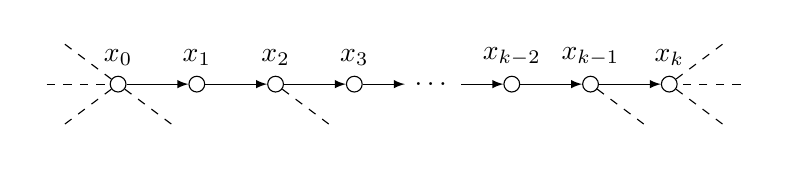
\begin{tikzpicture}
    [
    point/.style={circle,draw,inner sep=0pt,minimum size=2mm},
    ]
    \node (1) at (0,1) [point,label=above:$x_0$] {};
    \node (2) at (1,1) [point,label=above:$x_1$] {};
    \node (3) at (2,1) [point,label=above:$x_2$] {};
    \node (4) at (3,1) [point,label=above:$x_3$] {};
    \node (dots) at (4,1) [] {\dots};
    \node (k2) at (5,1) [point,label=above:$x_{k-2}$] {};
    \node (k1) at (6,1) [point,label=above:$x_{k-1}$] {};
    \node (k) at (7,1) [point,label=above:$x_k$] {};
    \draw [-latex] (1) to (2);
    \draw [-latex] (2) to (3);
    \draw [-latex] (3) to (4);
    \draw [-latex] (4) to (dots);
    \draw [-latex] (dots) to (k2);
    \draw [-latex] (k2) to (k1);
    \draw [-latex] (k1) to (k);

    \node (e1) [above left=4mm and 6mm of 1]  {};
    \node (e2) [left=8mm of 1] {};
    \node (e3) [below left=4mm and 6mm of 1] {};
    \node (e4) [above right=4mm and 6mm of k] {};
    \node (e5) [right=8mm of k] {};
    \node (e6) [below right=4mm and 6mm of k] {};
    \draw [dashed] (e1) to (1);
    \draw [dashed] (e2) to (1);
    \draw [dashed] (e3) to (1);
    \draw [dashed] (e4) to (k);
    \draw [dashed] (e5) to (k);
    \draw [dashed] (e6) to (k);

    \node (b1) [below right=4mm and 6mm of 1] {};
    \node (b3) [below right=4mm and 6mm of 3] {};
    \node (bk1) [below right=4mm and 6mm of k1] {};
    \draw [dashed] (1) to (b1);
    \draw [dashed] (3) to (b3);
    \draw [dashed] (k1) to (bk1);
  \end{tikzpicture}
\]
In the above graph, only every other vertex are restricted to only have one successor.
We will call this path variant an \textit{oddly trimmed path}, and define it formally as follows:
A path $\langle x_0,x_k\rangle$\todo{This notation is not explained} is oddly trimmed if for each odd $i < k$, $N(x_i) = \{x_{i+1}\}$.
One can immediately note that any fully trimmed path is also oddly trimmed.

The axioms we get from the oddly trimmed path above does not differ significantly from the fully trimmed variant.
Since the vertices $x_0, x_2, x_4, \dots ,x_{k_1}$ no longer have single successors, their corresponding OR-clauses will no longer be binary.
However, since none of these OR-clauses are used in the above proof, the proof will remain valid also for the oddly trimmed path.

We can thus generalize further and say that any two vertices connected by an oddly trimmed path of odd length is vel-connected.

	% !TEX root= ../main.tex
\externaldocument{../proofs/vels}
\externaldocument{odd_paths}
\section{Odd vels}
\label{sec:Odd vels}
The following observation will further generalize the concept of oddly trimmed paths:

The direction of edges in a graph can often be changed individually while still keeping many axiomatic clauses unchanged, including all the NAND-clauses.

Consider the following graph:\par
\begin{figure}[!h]
  \centering
  \begin{tikzpicture}
    [
    point/.style={circle,draw,inner sep=0pt,minimum size=2mm}
    ]
    \node (x0) at (0,3) [point, label=above:$x_0$] {};
    \node (x1) at (1,2) [point, label=above:$x_1$] {};
    \node (x2) at (2,1) [point, label=above:$x_2$] {};
    \node (x3) at (3,0) [point, label=above:$x_3$] {};
    \node (x4) at (4,1) [point, label=above:$x_4$] {};
    \node (x5) at (5,2) [point, label=above:$x_5$] {};
    \draw [-latex] (x0) to (x1);
    \draw [-latex] (x1) to (x2);
    \draw [-latex] (x2) to (x3);
    \draw [-latex] (x4) to (x3);
    \draw [-latex] (x5) to (x4);

    \node (e1) [below left=6mm and 4mm of x3]  {};
    \node (e2) [below=8mm of x3] {};
    \node (e3) [below right=6mm and 4mm of x3] {};
    \draw [dashed] (e1) to (x3);
    \draw [dashed] (e2) to (x3);
    \draw [dashed] (e3) to (x3);

    \node (b0) [below left=6mm and 4mm of x0] {};
    \node (b2) [below left=6mm and 4mm of x2] {};
    \node (b5) [below right=6mm and 4mm of x5] {};
    \draw [dashed] (x0) to (b0);
    \draw [dashed] (x2) to (b2);
    \draw [dashed] (x5) to (b5);
  \end{tikzpicture}
  \caption{}
  \label{fig:vel-example}
\end{figure}
\FloatBarrier
From the above graph, $\ol{x_0x_5}$ can be proven in the same way as in the proof of $\ol{x_0x_9}$ in Figure~\ref{fig:proof_x0x9}.
Again, the only thing we are changing in terms of the axioms are the OR-clauses that are not used in the proof.

We will call this kind of graph structure an \textit{odd vel} and define it formally in the following way:
\begin{definition}
  Two vertices $a$ and $b$ have an \textit{odd vel} between them if there exists a vertex $c$ such that there are oddly trimmed paths from $a$ to $c$ and from $b$ to $c$, one of even length (possibly 0) and one of odd length.
\end{definition}
Notice that an oddly trimmed path of odd length is just an instance of an odd vel where the even path is of length 0.

The formal proof why all NAND-clauses from vertices connected by such vels are provable in Neg can be found in Section~\ref{sec:Provability of NAND-clauses from vels}.

There are obviously other ways of altering directions of individual edges in a path.
The next example will however show that most of them will alter the OR-clauses in such a way that implication (1) no longer hold.

\begin{figure}[!h]
  \centering
  \begin{tikzpicture}
    [
    point/.style={circle,draw,inner sep=0pt,minimum size=2mm},
    one/.style={fill=black},
    ]
    \node (x0) at (0,1) [point, one, label=above:$a$] {};
    \node (x1) at (1,2) [point] {};
    \node (x2) at (2,1) [point] {};
    \node (x3) at (3,0) [point, one, label=above:$b$] {};
    \draw [-latex] (x1) to (x0);
    \draw [-latex] (x1) to (x2);
    \draw [-latex] (x2) to (x3);

    \node (e1) [below left=6mm and 4mm of x0]  {};
    \node (e2) [below=8mm of x0] {};
    \node (e3) [below right=6mm and 4mm of x0] {};
    \draw [dashed] (e1) to (x0);
    \draw [dashed] (e2) to (x0);
    \draw [dashed] (e3) to (x0);

    \node (e1) [below left=6mm and 4mm of x3]  {};
    \node (e2) [below=8mm of x3] {};
    \node (e3) [below right=6mm and 4mm of x3] {};
    \draw [dashed] (e1) to (x3);
    \draw [dashed] (e2) to (x3);
    \draw [dashed] (e3) to (x3);
  \end{tikzpicture}
  \hspace{5mm}
  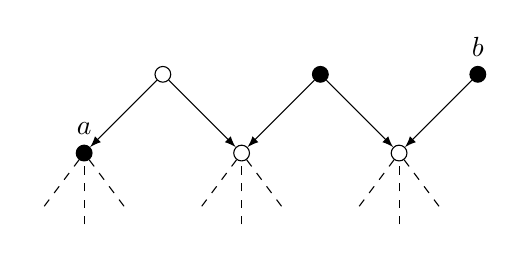
\begin{tikzpicture}
    [
    point/.style={circle,draw,inner sep=0pt,minimum size=2mm},
    one/.style={fill=black},
    ]
    \node (x0) at (0,1) [point, one, label=above:$a$] {};
    \node (x1) at (1,2) [point] {};
    \node (x2) at (2,1) [point] {};
    \node (x3) at (3,2) [point, one] {};
    \node (x4) at (4,1) [point] {};
    \node (x5) at (5,2) [point, one, label=above:$b$] {};

    \draw [-latex] (x1) to (x0);
    \draw [-latex] (x1) to (x2);
    \draw [-latex] (x3) to (x2);
    \draw [-latex] (x3) to (x4);
    \draw [-latex] (x5) to (x4);

    \node (e1) [below left=6mm and 4mm of x0]  {};
    \node (e2) [below=8mm of x0] {};
    \node (e3) [below right=6mm and 4mm of x0] {};
    \draw [dashed] (e1) to (x0);
    \draw [dashed] (e2) to (x0);
    \draw [dashed] (e3) to (x0);

    \node (e1) [below left=6mm and 4mm of x2]  {};
    \node (e2) [below=8mm of x2] {};
    \node (e3) [below right=6mm and 4mm of x2] {};
    \draw [dashed] (e1) to (x2);
    \draw [dashed] (e2) to (x2);
    \draw [dashed] (e3) to (x2);

    \node (e1) [below left=6mm and 4mm of x4]  {};
    \node (e2) [below=8mm of x4] {};
    \node (e3) [below right=6mm and 4mm of x4] {};
    \draw [dashed] (e1) to (x4);
    \draw [dashed] (e2) to (x4);
    \draw [dashed] (e3) to (x4);
  \end{tikzpicture}
  \caption{}
  \label{fig:inverse-vel}
\end{figure}
\FloatBarrier
The figure above shows two odd paths that have had some of their edges flipped.
In both examples, the shown kernels contain both $a$ and $b$, showing that neither of these constructions are providing a provable NAND-clause $\ol{ab}$ in Neg.

	% !TEX root= ../main.tex
\externaldocument{general_trimming}
\externaldocument{odd_paths}
\externaldocument{odd_vels}
\section{Inductive definitions}
\label{sec:Inductive definitions}
All the graph structures presented in this chapter so far can easily be defined inductively.
For instance, given some graph $\mathbf{G}=(G,N)$, let $V_1 \subseteq G \times G$ denote the set of all pairs of vertices related by our original vel-definition (Definition~\ref{def:vel}) where `trimmed' meant strictly non-branching.

We can define $V_1$ inductively in the following way, with $a$ and $b$ being arbitrary vertices from $G$.
\begin{align}
  \textbf{(BC):}&\quad N(a,b) \vee N(b,a) &\Rightarrow  V_1(a,b)\\
  \textbf{(IS):}&\quad \exists c \in N(a): (N(c) =\{d\} \wedge V_1(d,b)) &\Rightarrow V_1(a,b)
\end{align}
The symmetry in the base case is what makes this a definition of a vel and not a path, while the trimmed-ness gets expressed by the restrictions we set on vertex $c$.

\subsection{The $V_2$ construction}
\label{sub:The V2 construction}
It is now  much easier to formally express the new, weaker concept of trimming.
Let $V_2 \subseteq G \times G$ be the set of all pairs of vertices related by our new vel-definition.
$V_2$ can be defined inductively in the following way, again with $a$ and $b$ as arbitrary vertices from $G$.
\begin{align}
  \textbf{(BC):}&\quad N(a,b) \vee N(b,a) &\Rightarrow V_2(a,b)\label{eq:V2_BC}\\
  \textbf{(IS):}&\quad \exists c \in N(a):
  \left ( \begin{tabular}{l}
  $\exists d \in N(c): V_2(d,b) \quad \wedge$\\
  $\forall d \in N(c): V_2(d,b) \vee V_2(d,a) \vee V_2(d,d)$
  \end{tabular} \right )
  &\Rightarrow V_2(a,b)\label{eq:V2_IS}
\end{align}
Comparing the two inductive definitions, it is easy to see that $V_2$ is a generalization of $V_1$.

The fact that $V_2(a,b) \;\Rightarrow\; \vdash \ol{ab}$ can now be proven inductively, showing that $V_2$ satisfies implication (1):
\begin{proof}
  Given a graph $G$ with two vertices $a$ and $b$ such that $V_2(a,b)$:

  Base case:
  If $N(a,b)$ or $N(b,a)$, then the NAND-clause $\ol{ab}$ will be an axiom and thus trivially provable.

  Inductive step:
  The existence of a vertex $c \in N(a)$ gives us that the NAND-clause $\ol{ac}$ is an axiom.
  Letting $D$ denoting the set $N(c)$ we also have that the OR-clause $cD$ is an axiom.
  This gives us the following incomplete proof:\par
  \begin{figure}[!h]
    \centering
    \begin{prooftree*}
      \Hypo{\ol{ac}}
      \Hypo{\dots}
      \Infer[right label=$cD$]2{\ol{ab}}
    \end{prooftree*}
    \caption{}
    \label{fig:proof_v2_partial}
  \end{figure}
  \FloatBarrier
  Let $D_b$, $D_a$ and $D_d$ be subsets of $D$ such that for any $d \in D$:
  \begin{align}
    d \in D_b \Leftrightarrow V_2(d,b),\quad d \in D_a \Leftrightarrow V_2(d,a),\quad d \in D_d \Leftrightarrow V_2(d,d)
  \end{align}
  The current situation is illustrated in Figure~\ref{fig:v2_situation}\par
  \begin{figure}[!h]
    \centering
    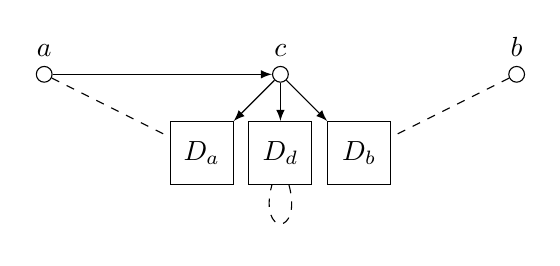
\begin{tikzpicture}
      [
      point/.style={circle,draw,inner sep=0pt,minimum size=2mm},
      collection/.style={rectangle,draw,inner sep=0pt,minimum height=8mm, minimum width= 8mm}
      ]
      \node (a) at (0,1) [point, label=above:$a$] {};
      \node (b) at (6,1) [point, label=above:$b$] {};
      \node (c) at (3,1) [point, label=above:$c$] {};
      \node (Da) at (2,0) [collection] {$D_a$};
      \node (Db) at (4,0) [collection] {$D_b$};
      \node (Dd) at (3,0) [collection] {$D_d$};
      \draw [-latex] (c) to (Da);
      \draw [-latex] (a) to (c);
      \draw [-latex] (c) to (Db);
      \draw [-latex] (c) to (Dd);
      \draw [dashed] (a) to (Da);
      \draw [dashed] (b) to (Db);
      \draw [dashed, loop below] (Dd) to (Dd);
    \end{tikzpicture}
    \caption{The inductive case of a $V_2$ construction.
    Boxes represents sets of vertices.
    An edge between a vertex and a box represents a set of edges from the vertex to each of the vertices in the set.}
    \label{fig:v2_situation}
  \end{figure}
  \FloatBarrier
  The inductive part of the $V_2$ definition (\ref{eq:V2_IS}) reveals two properties of the sets $D_b$, $D_a$ and $D_d$:
  \begin{itemize}
    \item The set $D_b$ is nonempty, since $\exists d \in N(c): V_2(d,b)$.
    \item $D_b \cup D_a \cup D_d = D$, since $\forall d \in N(c): V_2(d,b) \vee V_2(d,a) \vee V_2(d,d)$.
  \end{itemize}
  The induction hypothesis lets us assume the provability of the following sets of NAND-clauses:
  $\{ \ol{db} \;|\; d \in D_b \},\{ \ol{da} \;|\; d \in D_a \},\{ \ol{d} \;|\; d \in D_d \}$.
  Inserting these clauses into the incomplete proof from Figure~\ref{fig:proof_v2_partial} results the following proof:\par
  \begin{figure}[!h]
    \centering
    \begin{prooftree*}
      \Hypo{\ol{ac}}
      \Hypo{ \{ \ol{db} \;|\; d \in D_b \} }
      \Hypo{ \{ \ol{da} \;|\; d \in D_a \} }
      \Hypo{ \{ \ol{d} \;|\; d \in D_d \} }
      \Infer[right label=$cD$]4{\ol{ab}}
    \end{prooftree*}
    \caption{}
    \label{fig:proof_v2}
  \end{figure}
  The nonemptiness of $D_b$ gives us the existence of a $b$ in the premise, while he fact that $D_b \cup D_a \cup D_d = D$ guarantees that each atom in the OR-clause $D$ has a match in a NAND-clause.

  The proof is thus valid, finishing the inductive step and ultimately proving the fact that $V_2(a,b) \Rightarrow \;\vdash \ol{ab}$.
\end{proof}
Having that $V_2$ satisfies implication (1), if one could show that it also satisfies implication (2), the consequences would be considerable.
It would mean that any provable binary NAND-clause would have a proof that in each step combined a set of already proved binary NAND-clauses with an axiom.
Any provable NAND-clause could in other words be constructed by adding one fresh axiom at every step, hinting at a possible normal form of proofs in Neg.

Unfortunately, $V_2$ does \textit{not} satisfy implication (2).
The vertices $a$ and $b$ in the graph presented below will not be related by $V_2$, but $\ol{ab}$ is still provable in Neg.
The graph will thus act as a counterexample for implication (2).\par
\begin{figure}[!h]
  \centering
  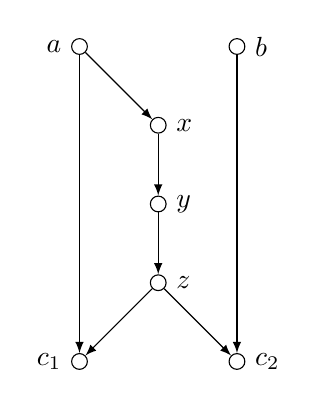
\begin{tikzpicture}
    [
    point/.style={circle,draw,inner sep=0pt,minimum size=2mm}
    ]
    \node (a) at (0,4) [point, label=left:$a$] {};
    \node (x) at (1,3) [point, label=right:$x$] {};
    \node (y) at (1,2) [point, label=right:$y$] {};
    \node (z) at (1,1) [point, label=right:$z$] {};
    \node (c1) at (0,0) [point, label=left:$c_1$] {};
    \node (c2) at (2,0) [point, label=right:$c_2$] {};
    \node (b) at (2,4) [point, label=right:$b$] {};
    \draw [-latex] (a) to (c1);
    \draw [-latex] (a) to (x);
    \draw [-latex] (x) to (y);
    \draw [-latex] (y) to (z);
    \draw [-latex] (z) to (c1);
    \draw [-latex] (z) to (c2);
    \draw [-latex] (b) to (c2);
  \end{tikzpicture}
  \caption{}
  \label{fig:v2_counter_graph}
\end{figure}
\FloatBarrier
Given the above graph, $\ol{ab}$ can be proven like follows:\par
\begin{figure}[!h]
  \centering
  \begin{prooftree*}
    \Hypo{\ol{ax}}
    \Hypo{\ol{yz}}
    \Infer[left label=$xy$]2{\ol{az}}
    \Hypo{\ol{ac_1}}
    \Hypo{\ol{bc_2}}
    \Infer[right label=$zc_1c_2$]3{\ol{ab}}
  \end{prooftree*}
  \caption{}
  \label{fig:v2_counter_proof}
\end{figure}
To show that the graph in Figure~\ref{fig:v2_counter_graph} is not an instance of $V_2$ demands a closer look at the graph.

Assume $V_2(a,b)$.
Since $a$ and $b$ are not connected by an edge, their relation has to be an instance of the inductive step.
Because of the nonemptiness requirement, $\exists c \in N(a):\exists d \in N(c): V_2(d,b)$ from the $V_2$ defintion, either $a$  must have a successor $c$ which again has a successor $d$ such that $V_2(d,b)$ or $b$ must have a successor $c$ which again has a successor $d$ such that $V_2(d,a)$.

The vertices $a$ and $b$ have a total of 3 successors, 2 of which are sinks and therefore unable to satisfy the nonemptiness requirement.
The last successor is the vertex $x$, which only has one successor, vertex $y$.\par
\begin{figure}[!h]
  \centering
  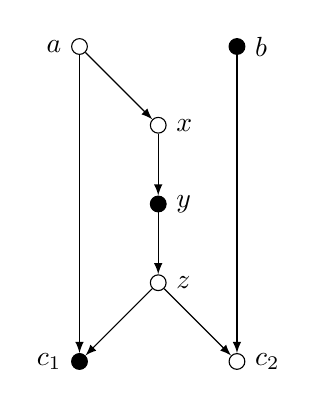
\begin{tikzpicture}
    [
    point/.style={circle,draw,inner sep=0pt,minimum size=2mm},
    one/.style={fill=black}
    ]
    \node (a) at (0,4) [point, label=left:$a$] {};
    \node (x) at (1,3) [point, label=right:$x$] {};
    \node (y) at (1,2) [point,one, label=right:$y$] {};
    \node (z) at (1,1) [point, label=right:$z$] {};
    \node (c1) at (0,0) [point,one, label=left:$c_1$] {};
    \node (c2) at (2,0) [point, label=right:$c_2$] {};
    \node (b) at (2,4) [point,one, label=right:$b$] {};
    \draw [-latex] (a) to (c1);
    \draw [-latex] (a) to (x);
    \draw [-latex] (x) to (y);
    \draw [-latex] (y) to (z);
    \draw [-latex] (z) to (c1);
    \draw [-latex] (z) to (c2);
    \draw [-latex] (b) to (c2);
  \end{tikzpicture}
  \caption{}
  \label{fig:v2_counter_assignment}
\end{figure}
\FloatBarrier
The above solution shows us by soundness of Neg that $\ol{yb}$ is unprovable, and therefore by implication (1) that $y$ and $b$ cannot be $V_2$-related.
Since none of the successors of $a$ and $b$ satisfies the nonemptiness requirement, they also are not $V_2$ related.
We can therefore conclude that $V_2$ does not satisfy implication (2).

\subsection{The $V_3$ construction}
\label{sub:The V3 construction}
Now, in what way can $V_2$ be generalized in order to include the graph in Figure~\ref{fig:v2_counter_graph}?
Looking at the proof in Figure~\ref{fig:proof_v2}, we see that the axiomatic NAND-clause $\ol{ac}$ is a crucial part of the premise, representing the $c \in N(a)$ in the definition of $V_2$.
Observe that a case where $\ol{ac}$ is non-axiomatic would not invalidate this rule application.
In other words, the vertex $c$ from the $V_2$ definition does not necessarily need to be in the neighborhood of $a$, they only need to be in a $V_2$-relation.

Based on this observation, we define the construction $V_3$ which is a generalization of $V_2$.
Like in the definitions of $V_1$ and $V_2$, $a$ and $b$ are vertices from $G$.
\begin{align}
  \textbf{(BC):}&\quad N(a,b) \vee N(b,a) &\Rightarrow V_3(a,b)\label{eq:V3_BC}\\
  \textbf{(IS):}&\quad \exists c \in G:
  \left ( \begin{tabular}{l}
  $\exists d \in N(c) \cup \{ c \} : V_3(d,a) \quad \wedge$\\
  $\exists d \in N(c) \cup \{ c \} : V_3(d,b) \quad \wedge$\\
  $\forall d \in N(c) \cup \{ c \} : V_3(d,a) \vee V_3(d,b) \vee V_3(d,d)$
  \end{tabular} \right )
  &\Rightarrow V_3(a,b)\label{eq:V3_IS}
\end{align}
$V_2$ required $a$ to have an edge to $c$.
We are now treating $c$ just like its successors by requiring it to be in $V_3$-relation to either $a$, $b$ or itself.
Requiring $a$ to be in $V_3$-relation to some vertex in $N(c) \cup \{ c \}$ is now what ensures the inclusion of $a$ in the proof.

Looking back at the graph from Figure~\ref{fig:v2_counter_graph}, we see that vertex $z$ is clearly $V_3$-related to $a$ while its successors, $c_1$ and $c_2$, are $V_3$-related to $a$ and $b$, respectively.
The vertices $a$ and $b$ are thus $V_3$-related.

Implication (1) for $V_3$ is proven in more or less the same way as we proved implication (1) for $V_2$ in Section~\ref{sub:The V2 construction}.
Therefore, only a condenced version will be shown here:
\begin{proof}
  Given a graph $G$ with two vertices $a$ and $b$ such that $V_3(a,b)$:

  Base case: Same as in $V_2$ proof.

  Inductive step: Let $D = N(c) \cup \{ c \}$ and let $D_a$, $D_b$ and $D_d$ denote the same sets as in the $V_2$ proof.
  The definition of $V_3$ tells us that both $D_a$ and $D_b$ are nonempty.
  This fact together with the fact that $D = D_a \cup D_b \cup D_d$ lets us form the following proof:\par
  \begin{figure}[!h]
    \centering
    \begin{prooftree*}
      \Hypo{ \{ \ol{da} \;|\; d \in D_a \} }
      \Hypo{ \{ \ol{db} \;|\; d \in D_b \} }
      \Hypo{ \{ \ol{d} \;|\; d \in D_d \} }
      \Infer[right label=$D$]3{\ol{ab}}
    \end{prooftree*}
    \caption{}
    \label{fig:proof_v3}
  \end{figure}
  No assumptions was made on the vertices $a$ and $b$, so we can conclude that $V_3(a,b)~\Rightarrow~\;\vdash~\ol{ab}$.
\end{proof}
\subsection{$V_3$ and implication (2)}
\label{sub:V3 and implication 2}
Just like with $V_2$, if $V_3$ also satisfies implication (2), it has some considerable consequences for our proof system, Neg.
Figure~\ref{fig:proof_v3} shows that if two vertices $a$ and $b$ are $V_3$-related, not only is $\ol{ab}$ provable in Neg, it is provable in such a way that the premise of the last rule application contains binary NAND-clauses only (the proof has a \textit{binary root}).

If $V_3$ satisfies implication (1) and (2), then for any provable binary NAND-clause $\ol{ab}$, by implication (1) and (2), it has a proof with a binary root.
Applying now the same reasoning on all of the binary NAND-clauses in its premise, we get that all of these also have proofs with binary roots.
Doing this repeatedly throughout the whole proof of $\ol{ab}$ ultimately gives us a proof containing exclusively binary NAND-clauses.
Implication (2) thus gives us that for any provable binary NAND-clause there exists a proof in Neg with binary NAND-clauses only.
We will however see that implication (2) does \textit{not} hold for $V_3$.\par

The graph in Figure~\ref{fig:v3_counter_graph} provides a provable NAND-clause $\ol{ab}$, but is not an instance of $V_3$.

The graph is admittedly a bit over-simplified.
Even though the vertices $y_1$, $y_2$ and $c_2$ are depicted like sinks, we will be treating them as initial vertices of (non-depicted) disjoint rays.
We will however not consider the clauses corresponding to the elements of these rays, since these are not going to contribute to our argument.
\begin{figure}[!h]
  \centering
  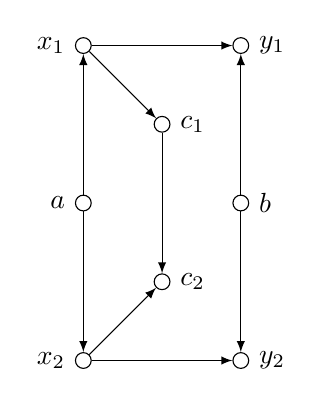
\begin{tikzpicture}
    [
    point/.style={circle,draw,inner sep=0pt,minimum size=2mm}
    ]
    \node (a) at (0,2) [point,label=left:$a$] {};
    \node (x1) at (0,4) [point,label=left:$x_1$] {};
    \node (x2) at (0,0) [point,label=left:$x_2$] {};
    \node (b) at (2,2) [point,label=right:$b$] {};
    \node (y1) at (2,4) [point,label=right:$y_1$] {};
    \node (y2) at (2,0) [point,label=right:$y_2$] {};
    \node (c1) at (1,3) [point,label=right:$c_1$] {};
    \node (c2) at (1,1) [point,label=right:$c_2$] {};
    \draw [-latex] (a) to (x1);
    \draw [-latex] (a) to (x2);
    \draw [-latex] (b) to (y1);
    \draw [-latex] (b) to (y2);
    \draw [-latex] (x1) to (y1);
    \draw [-latex] (x1) to (c1);
    \draw [-latex] (x2) to (y2);
    \draw [-latex] (x2) to (c2);
    \draw [-latex] (c1) to (c2);
  \end{tikzpicture}
  \caption{}
  \label{fig:v3_counter_graph}
\end{figure}
\FloatBarrier
Here is one way to prove $\ol{ab}$ in Neg given the graph theory from Figure~\ref{fig:v3_counter_graph}:\par
\begin{figure}[!h]
  \centering
  \begin{prooftree*}
    \Hypo{\ol{ax_2}}
    \Hypo{\ol{by_2}}
    \Hypo{\ol{c_1c_2}}
    \Infer[left label = $x_2y_2c_2$]3{\ol{abc_1}}
    \Hypo{\ol{ax_1}}
    \Hypo{\ol{by_1}}
    \Hypo{\ol{c_1c_2}}
    \Infer[right label = $x_1y_1c_1$]3{\ol{abc_2}}
    \Infer[left label = $c_1c_2$]2{\ol{ab}}
  \end{prooftree*}
  \caption{}
  \label{fig:v3_counter_proof}
\end{figure}
\FloatBarrier
Now, if implication (2) holds for $V_3$, we would expect $a$ and $b$ to be $V_3$-related in the above graph.
In other words, we would expect there to be a third vertex in the graph such that it and each of its successors are $V_3$-related to either $a$, $b$ or itself and such that there is at least one
This can be shown to be impossible.

Consider the following six solutions of the graph:\par
\begin{figure}[!h]
  \centering
  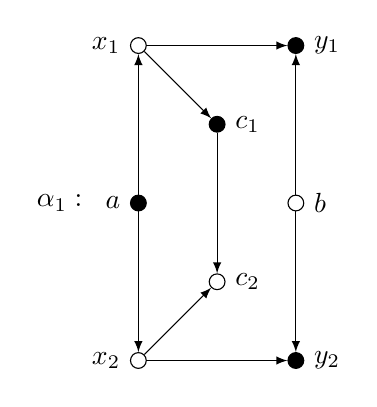
\begin{tikzpicture}
    [
    point/.style={circle,draw,inner sep=0pt,minimum size=2mm},
    one/.style={fill=black},
    collection/.style={thick,rectangle,draw,inner sep=0pt,minimum height=14mm, minimum width= 9mm}
    ]
    \node (label) at (-1,2) {$\alpha_1:$};
    \node (a) at (0,2) [point, one,label=left:$a$] {};
    \node (x1) at (0,4) [point,label=left:$x_1$] {};
    \node (x2) at (0,0) [point,label=left:$x_2$] {};
    \node (b) at (2,2) [point,label=right:$b$] {};
    \node (y1) at (2,4) [point, one,label=right:$y_1$] {};
    \node (y2) at (2,0) [point, one,label=right:$y_2$] {};
    \node (c1) at (1,3) [point, one,label=right:$c_1$] {};
    \node (c2) at (1,1) [point,label=right:$c_2$] {};
    \draw [-latex] (a) to (x1);
    \draw [-latex] (a) to (x2);
    \draw [-latex] (b) to (y1);
    \draw [-latex] (b) to (y2);
    \draw [-latex] (x1) to (y1);
    \draw [-latex] (x1) to (c1);
    \draw [-latex] (x2) to (y2);
    \draw [-latex] (x2) to (c2);
    \draw [-latex] (c1) to (c2);
  \end{tikzpicture}
  \hspace{5mm}
  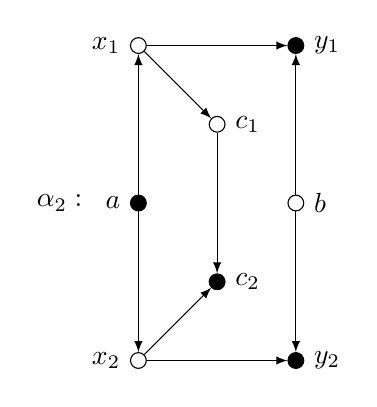
\begin{tikzpicture}
    [
    point/.style={circle,draw,inner sep=0pt,minimum size=2mm},
    one/.style={fill=black},
    collection/.style={thick,rectangle,draw,inner sep=0pt,minimum height=14mm, minimum width= 9mm}
    ]
    \node (label) at (-1,2) {$\alpha_2:$};
    \node (a) at (0,2) [point, one,label=left:$a$] {};
    \node (x1) at (0,4) [point,label=left:$x_1$] {};
    \node (x2) at (0,0) [point,label=left:$x_2$] {};
    \node (b) at (2,2) [point,label=right:$b$] {};
    \node (y1) at (2,4) [point, one,label=right:$y_1$] {};
    \node (y2) at (2,0) [point, one, label=right:$y_2$] {};
    \node (c1) at (1,3) [point,label=right:$c_1$] {};
    \node (c2) at (1,1) [point, one, label=right:$c_2$] {};
    \draw [-latex] (a) to (x1);
    \draw [-latex] (a) to (x2);
    \draw [-latex] (b) to (y1);
    \draw [-latex] (b) to (y2);
    \draw [-latex] (x1) to (y1);
    \draw [-latex] (x1) to (c1);
    \draw [-latex] (x2) to (y2);
    \draw [-latex] (x2) to (c2);
    \draw [-latex] (c1) to (c2);
  \end{tikzpicture}
  \hspace{5mm}
  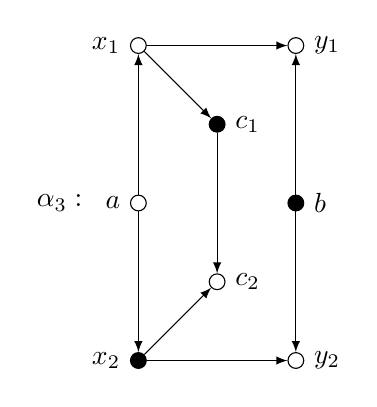
\begin{tikzpicture}
    [
    point/.style={circle,draw,inner sep=0pt,minimum size=2mm},
    one/.style={fill=black},
    collection/.style={thick,rectangle,draw,inner sep=0pt,minimum height=14mm, minimum width= 9mm}
    ]
    \node (label) at (-1,2) {$\alpha_3:$};
    \node (a) at (0,2) [point,label=left:$a$] {};
    \node (x1) at (0,4) [point,label=left:$x_1$] {};
    \node (x2) at (0,0) [point, one,label=left:$x_2$] {};
    \node (b) at (2,2) [point, one,label=right:$b$] {};
    \node (y1) at (2,4) [point,label=right:$y_1$] {};
    \node (y2) at (2,0) [point,label=right:$y_2$] {};
    \node (c1) at (1,3) [point, one,label=right:$c_1$] {};
    \node (c2) at (1,1) [point,label=right:$c_2$] {};
    \draw [-latex] (a) to (x1);
    \draw [-latex] (a) to (x2);
    \draw [-latex] (b) to (y1);
    \draw [-latex] (b) to (y2);
    \draw [-latex] (x1) to (y1);
    \draw [-latex] (x1) to (c1);
    \draw [-latex] (x2) to (y2);
    \draw [-latex] (x2) to (c2);
    \draw [-latex] (c1) to (c2);
  \end{tikzpicture}\\
  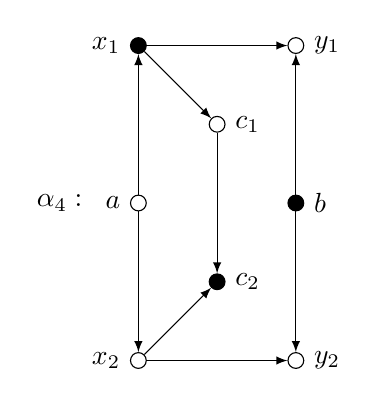
\begin{tikzpicture}
    [
    point/.style={circle,draw,inner sep=0pt,minimum size=2mm},
    one/.style={fill=black},
    collection/.style={thick,rectangle,draw,inner sep=0pt,minimum height=14mm, minimum width= 9mm}
    ]
    \node (label) at (-1,2) {$\alpha_4:$};
    \node (a) at (0,2) [point,label=left:$a$] {};
    \node (x1) at (0,4) [point, one,label=left:$x_1$] {};
    \node (x2) at (0,0) [point,label=left:$x_2$] {};
    \node (b) at (2,2) [point, one,label=right:$b$] {};
    \node (y1) at (2,4) [point,label=right:$y_1$] {};
    \node (y2) at (2,0) [point,label=right:$y_2$] {};
    \node (c1) at (1,3) [point,label=right:$c_1$] {};
    \node (c2) at (1,1) [point, one,label=right:$c_2$] {};
    \draw [-latex] (a) to (x1);
    \draw [-latex] (a) to (x2);
    \draw [-latex] (b) to (y1);
    \draw [-latex] (b) to (y2);
    \draw [-latex] (x1) to (y1);
    \draw [-latex] (x1) to (c1);
    \draw [-latex] (x2) to (y2);
    \draw [-latex] (x2) to (c2);
    \draw [-latex] (c1) to (c2);
  \end{tikzpicture}
  \hspace{5mm}
  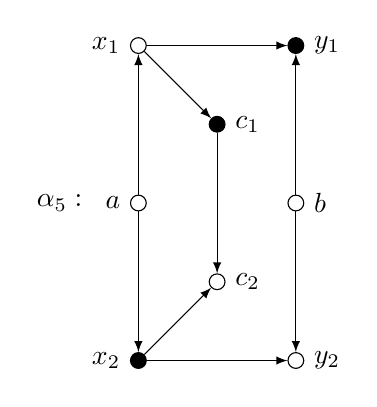
\begin{tikzpicture}
    [
    point/.style={circle,draw,inner sep=0pt,minimum size=2mm},
    one/.style={fill=black},
    collection/.style={thick,rectangle,draw,inner sep=0pt,minimum height=14mm, minimum width= 9mm}
    ]
    \node (label) at (-1,2) {$\alpha_5:$};
    \node (a) at (0,2) [point,label=left:$a$] {};
    \node (x1) at (0,4) [point,label=left:$x_1$] {};
    \node (x2) at (0,0) [point, one,label=left:$x_2$] {};
    \node (b) at (2,2) [point,label=right:$b$] {};
    \node (y1) at (2,4) [point, one, label=right:$y_1$] {};
    \node (y2) at (2,0) [point,label=right:$y_2$] {};
    \node (c1) at (1,3) [point, one,label=right:$c_1$] {};
    \node (c2) at (1,1) [point,label=right:$c_2$] {};
    \draw [-latex] (a) to (x1);
    \draw [-latex] (a) to (x2);
    \draw [-latex] (b) to (y1);
    \draw [-latex] (b) to (y2);
    \draw [-latex] (x1) to (y1);
    \draw [-latex] (x1) to (c1);
    \draw [-latex] (x2) to (y2);
    \draw [-latex] (x2) to (c2);
    \draw [-latex] (c1) to (c2);
  \end{tikzpicture}
  \hspace{5mm}
  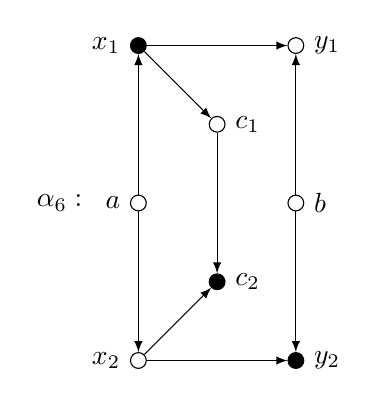
\begin{tikzpicture}
    [
    point/.style={circle,draw,inner sep=0pt,minimum size=2mm},
    one/.style={fill=black},
    collection/.style={thick,rectangle,draw,inner sep=0pt,minimum height=14mm, minimum width= 9mm}
    ]
    \node (label) at (-1,2) {$\alpha_6:$};
    \node (a) at (0,2) [point,label=left:$a$] {};
    \node (x1) at (0,4) [point, one, label=left:$x_1$] {};
    \node (x2) at (0,0) [point,label=left:$x_2$] {};
    \node (b) at (2,2) [point, label=right:$b$] {};
    \node (y1) at (2,4) [point,label=right:$y_1$] {};
    \node (y2) at (2,0) [point, one, label=right:$y_2$] {};
    \node (c1) at (1,3) [point,label=right:$c_1$] {};
    \node (c2) at (1,1) [point, one, label=right:$c_2$] {};
    \draw [-latex] (a) to (x1);
    \draw [-latex] (a) to (x2);
    \draw [-latex] (b) to (y1);
    \draw [-latex] (b) to (y2);
    \draw [-latex] (x1) to (y1);
    \draw [-latex] (x1) to (c1);
    \draw [-latex] (x2) to (y2);
    \draw [-latex] (x2) to (c2);
    \draw [-latex] (c1) to (c2);
  \end{tikzpicture}
  \caption{}
  \label{fig:v3_counter_solutions}
\end{figure}
\FloatBarrier
Given any pair of vertices $x,y$, if there exists an assignment such that $x$ and $y$ are both assigned 1, then $\ol{xy}$ is not provable in Neg.
We get this from soundness.

The table in Figure~\ref{fig:v3_counter_table} shows what pairs of vertices can be 1 under the samme assignment and thus constitute a binary NAND-clauses unprovable in Neg.
A cell is filled with a reference to the solution, if any, examplifying the case.
\begin{figure}[!h]
  \centering
  \[\begin{array}{|c||c|c|c|c|c|c|c|c|}
    \hline
    & a & b & x_1 & x_2 & y_1 & y_2 & c_1 & c_2 \\ \hline\hline
    a & \alpha_1 & & & & \alpha_1 & \alpha_1 & \alpha_1 & \alpha_2 \\ \hline
    b & & \alpha_4 & \alpha_4 & \alpha_3 & & & \alpha_3 & \alpha_4 \\ \hline
    x_1 & & & \alpha_4 & & & \alpha_6 & & \alpha_6 \\ \hline
    x_2 & & & & \alpha_5 & \alpha_5 & & \alpha_5 & \\ \hline
    y_1 & & & & & \alpha_1 & \alpha_1 & \alpha_1 & \alpha_2 \\ \hline
    y_2 & & & & & & \alpha_1 & \alpha_1 & \alpha_2 \\ \hline
    c_1 & & & & & & & \alpha_1 & \\ \hline
    c_2 & & & & & & & & \alpha_4 \\ \hline
  \end{array}\]
  \caption{}
  \label{fig:v3_counter_table}
\end{figure}
\FloatBarrier
Two important observations are to be made from the above table:

First, for each vertex in the graph, there exists a solution where that vertex is assigned 1.
By soundness, no unary NAND-clause can therefore be proven in Neg under this theory.

Secondly, among the pairs above that are not shown to be unprovable, only two are not axioms: $\ol{ab}$ and $\ol{x_1x_2}$.
We are thus left with the following collection of 11 ``not-unprovable'' binary NAND-clauses:
\begin{align}
  \{\; \ol{ab},\; \ol{ax_1},\; \ol{ax_2},\; \ol{by_1},\; \ol{by_2},\; \ol{x_1x_2},\; \ol{x_1y_1},\; \ol{x_1c_1},\; \ol{x_2y_2},\; \ol{x_2c_2} \; \ol{c_1c_2},\; \}
\end{align}
By the definition of $V_3$ from (\ref{eq:V2_BC}) and (\ref{eq:V2_IS}), in order for $a$ and $b$ to be $V_3$-related, a vertex $c$ has to exist such that it and all its successors are $V_3$-related to either $a$, $b$ or itself and such that at least one of them is $V_3$-related to $a$ and one to $b$.

It turns out that none of the vertices in the graph satisfies this requirement.

$a$ and $b$ are thus not $V_3$-related, even though $\ol{ab}$ is provable, so implication (2) fails.

	\chapter{Proof power of binary NAND-clauses}
	\label{chap:Proof power of binary NAND-clauses}
	% !TEX root= ../main.tex
In this chapter we will investigate the statement that whenever a theory is inconsistent, it can be proven in Neg using unary and binary NAND-clauses only.
Such a result would be significant both because it would be a strong property for a proof system to have in general, but also because it could potentially help us to further characterize a kernel-free graph

Having that any inconsistency can be proven in Neg using unary and binary NAND-clauses only, might imply a similar property in kernel-free graphs, namely that inconsistencies can be described as a collection of pairwise structural relations between vertices.

We will check the statement first for non-graph-based theories and then for theories based on graphs with different properties.

	% !TEX root= ../main.tex
\externaldocument{../binary_nands/motivation}
\section{Unrestricted theories}
\label{sec:Unrestricted theories}
This section will show that there exist inconsistencies in non-graph-based theories that are not possible to prove in Neg using only unary and binary NAND-clauses.
We will prove the pigeonhole principle to examplify this.

The pigeonhole principle states that whenever you have $n$ pigeons and $m$ holes such that $n > m$, then at least one hole must contain more than one pigeon.
We can prove this principle in Neg by proving an inconsistency of the theory that (1) all $n$ pigeons are contained in a hole and (2) each hole contains only one pigeon.

Letting the atom $x_i$ denote the pigeon $i$ occupying the hole $x$, the above theory, with $n$ pigeons and $m$ holes, can be formalized in the following way:
\begin{align}
  \text{(1):}\quad &\{ \; 1_i2_i3_i\dots m_i \;|\; i \leq n \; \}\\
  \text{(2):}\quad &\{ \; \ol{x_ix_j} \;|\; i < j \leq n, x \leq m \; \}
\end{align}
\subsection{Proof for 4 pigeons and 3 holes}
\label{sub:Proof for 4 pigeons and 3 holes}
The pigeonhole principle for 4 pigeons and 3 holes will have the following axioms:
\begin{align}
  \text{OR} &= \{ \; 1_12_13_1,\; 1_22_23_2,\; 1_32_33_3,\; 1_42_43_4 \; \} \label{eq:ax1}\\
  \text{NAND} &= \left \{
  \begin{tabular}{c}
    $\ol{1_11_2},\;\ol{1_11_3},\;\ol{1_11_4},\;\ol{1_21_3},\;\ol{1_21_4},\;\ol{1_31_4},$\\
    $\ol{2_12_2},\;\ol{2_12_3},\;\ol{2_12_4},\;\ol{2_22_3},\;\ol{2_22_4},\;\ol{2_32_4},$\\
    $\ol{3_12_2},\;\ol{3_13_3},\;\ol{3_13_4},\;\ol{3_23_3},\;\ol{3_23_4},\;\ol{3_33_4}$
  \end{tabular}
  \right \} \label{eq:ax2}
\end{align}

From the axioms above we can prove inconsistency in the following way:

Proving $\ol{1_4}$:
\begin{prooftree*}[separation=0.8em, rule margin=1ex]
  \Hypo{\ol{1_31_4}}
    \Hypo{\ol{1_21_4}}
    \Hypo{\ol{2_22_3}}
      \Hypo{\ol{1_11_4}}
      \Hypo{\ol{2_12_3}}
      \Hypo{\ol{3_13_2}}
    \Infer[right label = $1_12_13_1$]3{\ol{3_22_31_4}}
  \Infer[right label = $1_22_23_2$]3{\ol{2_31_4}}
    \Hypo{\ol{1_21_4}}
      \Hypo{\ol{1_11_4}}
      \Hypo{\ol{2_12_2}}
      \Hypo{\ol{3_13_3}}
    \Infer[right label = $1_12_13_1$]3{\ol{2_23_31_4}}
    \Hypo{\ol{3_23_3}}
  \Infer[right label = $1_22_23_2$]3{\ol{3_31_4}}
\Infer[right label = $1_32_33_3$, separation=0em]3{\ol{1_4}}
\end{prooftree*}

Proving $\ol{2_4}$:
\begin{prooftree*}[separation=0.8em, rule margin=1ex]
    \Hypo{\ol{1_21_3}}
    \Hypo{\ol{2_22_4}}
      \Hypo{\ol{1_11_3}}
      \Hypo{\ol{2_12_4}}
      \Hypo{\ol{3_13_2}}
    \Infer[right label = $1_12_13_1$]3{\ol{3_21_32_4}}
  \Infer[right label = $1_22_23_2$]3{\ol{1_32_4}}
  \Hypo{\ol{2_32_4}}
      \Hypo{\ol{1_11_2}}
      \Hypo{\ol{2_12_4}}
      \Hypo{\ol{3_13_3}}
    \Infer[left label = $1_12_13_1$]3{\ol{1_23_32_4}}
    \Hypo{\ol{2_22_4}}
    \Hypo{\ol{3_23_3}}
  \Infer[left label = $1_22_23_2$]3{\ol{3_32_4}}
\Infer[right label = $1_32_33_3$, separation=0em]3{\ol{2_4}}
\end{prooftree*}

Proving $\ol{3_4}$:
\begin{prooftree*}[separation=0.8em, rule margin=1ex]
    \Hypo{\ol{1_21_3}}
      \Hypo{\ol{1_11_3}}
      \Hypo{\ol{2_12_2}}
      \Hypo{\ol{3_13_4}}
    \Infer[left label = $1_12_13_1$]3{\ol{2_21_33_4}}
    \Hypo{\ol{3_23_4}}
  \Infer[left label = $1_22_23_2$]3{\ol{1_33_4}}
      \Hypo{\ol{1_11_2}}
      \Hypo{\ol{2_12_3}}
      \Hypo{\ol{3_13_4}}
    \Infer[left label = $1_12_13_1$]3{\ol{1_22_33_4}}
    \Hypo{\ol{2_22_3}}
    \Hypo{\ol{3_23_4}}
  \Infer[left label = $1_22_23_2$]3{\ol{2_33_4}}
  \Hypo{\ol{3_33_4}}
\Infer[left label = $1_32_33_3$, separation=0em]3{\ol{3_4}}
\end{prooftree*}

With these three unary clauses proven, we can now prove $\varnothing$ in one step:
\begin{prooftree*}[rule margin=1ex]
  \Hypo{\ol{1_4}}
  \Hypo{\ol{2_4}}
  \Hypo{\ol{3_4}}
  \Infer[left label = $1_42_43_4$]3{\varnothing}
\end{prooftree*}

Observe that NAND-clauses of length 3 appear several times in this proof.
We will show that this is unavoidable in Neg given the axioms from \ref{eq:ax1} and \ref{eq:ax2}
\subsection{Long NAND-clauses in pigeonhole proofs}
\label{sub:Long NAND-clauses in pigeonhole proofs}
As observed in \ref{sec:Motivation}, the only strategy in proving inconsistencies in Neg is to create new NAND-clauses until you have a set of unary NAND-clauses such that their union matches an OR-clause.

Now, what possible ways are there to create new NAND-clauses from our given pigeonhole axioms?
The OR-clauses are what dictates the ways new NAND-clauses can, be created, and since all OR-clauses are of length 3, we get that any premise must consist of exactly 3 NAND-clauses.
In addition, since all OR-clauses contain exactly one atom from each hole, each of the three NAND-clauses must contain atoms from different holes.

Looking at the NAND-clauses in the axiom set, we see that none of them contain atoms from two different holes, so the three axiomatic NAND-clauses eligible in a premise are mutually disjoint.
Since all three are binary, we have a total of 6 different axioms in the premise, and with the OR-clause shaving of 3 of these, our conclusion must contain 3 different atoms.
Any NAND-clause derived directly from axioms must therefore be of length 3.
\begin{prooftree*}
  \Hypo{\ol{1_i1_j}}
  \Hypo{\ol{2_i2_k}}
  \Hypo{\ol{3_i3_l}}
  \Infer[left label = $1_i2_i3_i$]3{\ol{1_j2_k3_l}}
\end{prooftree*}

It is easy to see that this generalizes to any version of the pigeonhole principle.
When you have $n$ holes and $>n$ pigeons, the OR-clauses will be of length $n$, requiring $n$ disjoint NAND-clauses in the premise, thus resulting in a NAND-clause of length $n$.

This means not only that we are unable to keep the clause length at 2, but also that the size of the clauses increase with the number of holes. 

	% !TEX root= ../main.tex
\section{Graph theories}
\label{sec:Graph theories}
We have just shown that in the case of unrestricted theories, there is no guarantee that an inconsistency is binary-derivable, but what about graph theories?
After all, it is the graph theories that motivated the conjecture in the first place.

It turns out that even for graph theories, some provable NAND-clauses require non-binary NAND-clauses in their proof, i.e they are \textit{not} binary-derivable.
This section will disprove the following conjecture:
\begin{conjecture}
  Given a graph theory, any provable binary NAND-clause is binary-derviable.
  \label{thm:non_binary_derivable}
\end{conjecture}
The conjecture will be disproven simply by presenting a graph containing a provable binary NAND-clause and show that the only way to prove it is through using non-binary NAND-clauses.
We will then make an attempt to extend the graph, making it inconsistent, and then show that its inconsistency proof has to include the non-binary-derivable NAND-clause.
This attempt will however prove to be unsuccessful.

Let us again consider the graph from Figure~\ref{fig:v3_counter_graph}, Section~\ref{sub:V3 and implication 2}:\par
\begin{figure}[!h]
  \centering
  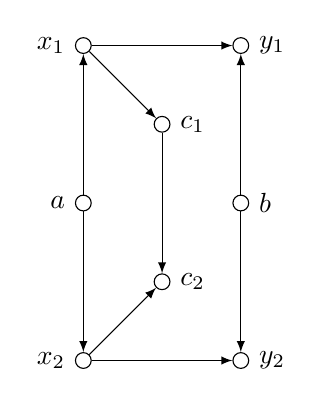
\begin{tikzpicture}
    [
    point/.style={circle,draw,inner sep=0pt,minimum size=2mm}
    ]
    \node (a) at (0,2) [point,label=left:$a$] {};
    \node (x1) at (0,4) [point,label=left:$x_1$] {};
    \node (x2) at (0,0) [point,label=left:$x_2$] {};
    \node (b) at (2,2) [point,label=right:$b$] {};
    \node (y1) at (2,4) [point,label=right:$y_1$] {};
    \node (y2) at (2,0) [point,label=right:$y_2$] {};
    \node (c1) at (1,3) [point,label=right:$c_1$] {};
    \node (c2) at (1,1) [point,label=right:$c_2$] {};
    \draw [-latex] (a) to (x1);
    \draw [-latex] (a) to (x2);
    \draw [-latex] (b) to (y1);
    \draw [-latex] (b) to (y2);
    \draw [-latex] (x1) to (y1);
    \draw [-latex] (x1) to (c1);
    \draw [-latex] (x2) to (y2);
    \draw [-latex] (x2) to (c2);
    \draw [-latex] (c1) to (c2);
  \end{tikzpicture}
  \caption{}
  \label{fig:open_door}
\end{figure}
As before, the vertices $y_1$, $y_2$ and $c_2$ are initial vertices of disjoint rays, and not sinks.

The NAND-clause we will show not to be binary-provable is $\ol{ab}$.
Figure~\ref{fig:v3_counter_proof} proves $\ol{ab}$, but the proof contains two non-binary NAND-clauses.
We will show that this is unavoidable.
In order to do this, we utilize the table from Figure~\ref{fig:v3_counter_table} worked out in Section~\ref{sub:V3 and implication 2}.
We will show it here for convenience.\par
\begin{figure}[!h]
  \centering
  \[\begin{array}{|c||c|c|c|c|c|c|c|c|}
    \hline
    & a & b & x_1 & x_2 & y_1 & y_2 & c_1 & c_2 \\ \hline\hline
    a & \alpha_1 & & & & \alpha_1 & \alpha_1 & \alpha_1 & \alpha_2 \\ \hline
    b &-& \alpha_4 & \alpha_4 & \alpha_3 & & & \alpha_3 & \alpha_4 \\ \hline
    x_1 &-&-& \alpha_4 & & & \alpha_6 & & \alpha_6 \\ \hline
    x_2 &-&-&-& \alpha_5 & \alpha_5 & & \alpha_5 & \\ \hline
    y_1 &-&-&-&-& \alpha_1 & \alpha_1 & \alpha_1 & \alpha_2 \\ \hline
    y_2 &-&-&-&-&-& \alpha_1 & \alpha_1 & \alpha_2 \\ \hline
    c_1 &-&-&-&-&-&-& \alpha_1 & \\ \hline
    c_2 &-&-&-&-&-&-&-& \alpha_4 \\ \hline
  \end{array}\]
  \caption{}
  \label{fig:open_door_table}
\end{figure}

Let us assume that we have a rule application with all binary NAND-clauses in the premise and with $\ol{ab}$ in the conclusion.
Based on the (Rneg)-rule, we know that the premise must contain at least one binary NAND-clause containg $a$ and at least one containing $b$.
The above table tells us that the only provable binary NAND-clauses that contain $a$ or $b$ are the ones in the axiom set:
$\ol{ax_1}$, $\ol{ax_2}$, $\ol{by_1}$ and $\ol{by_2}$.
Since we do not want any $x_i$ or $y_i$ in the conclusion, these variables have to be removed by the OR-clause.
The OR-clauses $x_1y_1c_1$ and $x_2y_2c_2$ are the only ones that contain both an $x$ and a $y$, making them the only OR-clauses that can potentially conclude with $\ol{ab}$.

This gives us the following information: since both the possible OR-clauses are of length 3, the rule application concluding with $\ol{ab}$ has 3 NAND-clauses in its premise; one containing an $x$, one containing a $y$ and one containing a $c$.
Looking at our table again, we see that the potentially provable NAND-clauses containing a $c$ are again the axioms only.
Since there are no provable NAND-clauses on the form $ac_i$ or $bc_i$, we get that the conclusion of our rule cannot possibly be of length 2, thus contradicting our assumption.
We can therefore conclude that $\ol{ab}$ is \textit{not} binary-derivable, thus disproving Conjecture~\ref{thm:non_binary_derivable}.
\subsection{Inconsistencies}
\label{sub:Inconsistencies}
We will to use the fact that some binary NAND-clauses are not binary-derivable in an attempt to show that some \textit{inconsistencies} are not binary-derivable.

The idea is to extend our original graph, making it inconsistent, but in such a way that $\varnothing$ can be proven only by using the NAND-clause $\ol{ab}$ somewhere in the proof.

Consider the following extension to our original graph from Figure~\ref{fig:open_door}:
\[
  \begin{tikzpicture}
    [
    point/.style={circle,draw,inner sep=0pt,minimum size=2mm},
    collection/.style={thick,rectangle,draw,inner sep=0pt,minimum height=14mm, minimum width= 9mm}
    ]
    \node (a) at (0,2) [point,label=left:$a$] {};
    \node (x1) at (0,4) [point,label=left:$x_1$] {};
    \node (x2) at (0,0) [point,label=left:$x_2$] {};
    \node (b) at (2,2) [point,label=right:$b$] {};
    \node (y1) at (2,4) [point,label=right:$y_1$] {};
    \node (y2) at (2,0) [point,label=right:$y_2$] {};
    \node (c1) at (1,3) [point,label=right:$c_1$] {};
    \node (c2) at (1,1) [point,label=right:$c_2$] {};
    \node (s) at (1,6) [point,label=left:$s$] {};
    \node (t) at (1,5) [point,label=below:$t$] {};
    \node (u1) at (-2,5) [point,label=left:$u_1$] {};
    \node (u2) at (4,5) [point,label=right:$u_2$] {};
    \draw [-latex] (a) to (x1);
    \draw [-latex] (a) to (x2);
    \draw [-latex] (b) to (y1);
    \draw [-latex] (b) to (y2);
    \draw [-latex] (x1) to (y1);
    \draw [-latex] (x1) to (c1);
    \draw [-latex] (x2) to (y2);
    \draw [-latex] (x2) to (c2);
    \draw [-latex] (c1) to (c2);
    \draw [-latex,loop right] (s) to (s);
    \draw [-latex] (s) to (t);
    \draw [-latex] (t) to (u1);
    \draw [-latex] (t) to (u2);
    \draw [-latex] (u1) to (a);
    \draw [-latex] (u2) to (b);
  \end{tikzpicture}
\]
The extension provides us with 6 new NAND-clauses and 4 new OR-clauses in the axioms set:
\begin{align}
  \text{OR'} &= \text{OR} \cup \{st,\; tu_1u_2,\; u_1a,\; u_2b \}\\
  \text{NAND'} &= \text{NAND} \cup \{\ol{s},\; \ol{st},\; \ol{tu_1},\; \ol{tu_2},\; \ol{u_1a},\; \ol{u_2b} \}
\end{align}

This extended graph can now be proven inconsistent using the newly provided clauses, as shown in the following Neg proof:
\begin{prooftree*}
  \Hypo{\ol{s}}
  \Hypo{\ol{tu_2}}
  \Hypo{\ol{tu_1}}
  \Hypo{\dots}
  \Infer1{\ol{ab}}
  \Infer[right label=$u_1a$]2{\ol{tb}}
  \Infer[right label=$u_2b$]2{\ol{t}}
  \Infer[right label=$st$]2{\varnothing}
\end{prooftree*}

We will now show that this inconsistency proof has to use the $\ol{ab}$ clause.

First of all, since both the vertices $s$ and $t$ are provably false, as the proof above shows, they can by soundness of Neg not be assigned 1 under any assignment.
This means that none of the binary NAND-clauses that contains either $s$ or $t$ can be ruled out as unprovable like we did above.

  \chapter{Proofs}
  \label{chap:Proofs}
  % !TEX root= ../main.tex
\section{Translating CNF to GNF}
\label{sec:Translating CNF to GNF}
Since any PL theory can be expressed in CNF, showing that any theory $P$ in CNF can be translated to a theory $R$ in GNF such that $P$ and $R$ are equisatisfiable gives us that any PL theory has an equisatisfiable GNF.

Given any CNF theory $P$, for each formula in it, follow the steps below to acquire its corresponding GNF theory.

\textbf{Step 1:}
For each literal $\neg x_i$ in the formula, introduce a fresh variable $x'_i$ and add the following two GNF formulae to $P$:
$x'_i \lar \neg x_i, x_i \lar \neg x'_i,$ (unless this has already been done while translating an earlier formula in the theory).

\textbf{Step 2:}
In each clause of the formula, replace every negative literal $\neg x_i$ with its corresponding $x'_i$ fom step 1.
Every clause in the formula does now contain positive literals only.

\textbf{Step 3:}
For every clause $(x_1 \vee x_2 \vee \dots \vee x_n)$, replace it with the following formula, where $y$ is fresh:
\[y \lar (\neg x_1 \wedge \neg x_2 \wedge \dots \wedge \neg x_n \wedge \neg y)\]

This formula is equisatisfiable with our original clause.

The combined set of all these acquired formulae will make up our GNF-theory.
We have only added proper GNF formulae and all variables appear to the left in exactly one clause, so $R$ will indeed be a GNF theory.

Step 1 is adding a bi-implication formula that is always satisfiable, since one of two variables in it is fresh.
One can think of it as a labelling of an already existing variable.
Thus, adding these formulae to a theory does not change its satisfiability/non-satisfiability.

Step 2 is replacing each negative literal with its label, also not changing the satisfiability.

Step 3 is replacing one formula with an equisatisfiable formula, thus not changing the overall satisfiability.

Since none of the steps above change the satisfiability of the theory, we can conclude that our acquired theory is equisatisfiable with to original CNF theory.

Below are some examples of CNF-theories with their corresponding GNF-theories.\\

\begin{example}
  \begin{align}
    \text{CNF:\quad}& ( a \vee b )\\
    \text{GNF:\quad}& ( a \lar \neg a'), (a' \lar \neg a), (b \lar \neg b'), (b' \lar \neg b), (y_1 \lar (\neg a \wedge \neg b \wedge \neg y_1))\\
    \\
    \text{CNF:\quad}& (\neg a)\\
    \text{GNF:\quad}& ( a \lar \neg a'), (a' \lar \neg a), (y_1 \lar (\neg a' \wedge \neg y_1))\\
  \end{align}
\end{example}

	\pagebreak
	% !TEX root= ../main.tex
\subsection{Inconsistency of Stretched Yablo}
\label{sub:Inconsistency of Stretched Yablo}

One variation of the Yablo-graph is the Stretched Yablo-graph, presented by Walicki in \cite{michal-completeness}.
While the Yablo-graph is a ray where each vertex on it has direct edges to all the vertices after it, the Stretched Yablo-graph is a ray where each vertex has \textit{disjoint paths} (with certain properties depending on the variation of Stretched Yablo) to all vertices in after it.

The variation on which we will be proving an inconsistency is one with a set of core vertices $\mathbb{N}$ where each vertex $x$ has a disjoint path to every vertex $y$ after it, such that the length of the path is $(2 \times (y - x) - 1)$.

\begin{figure}[!h]
  \centering
  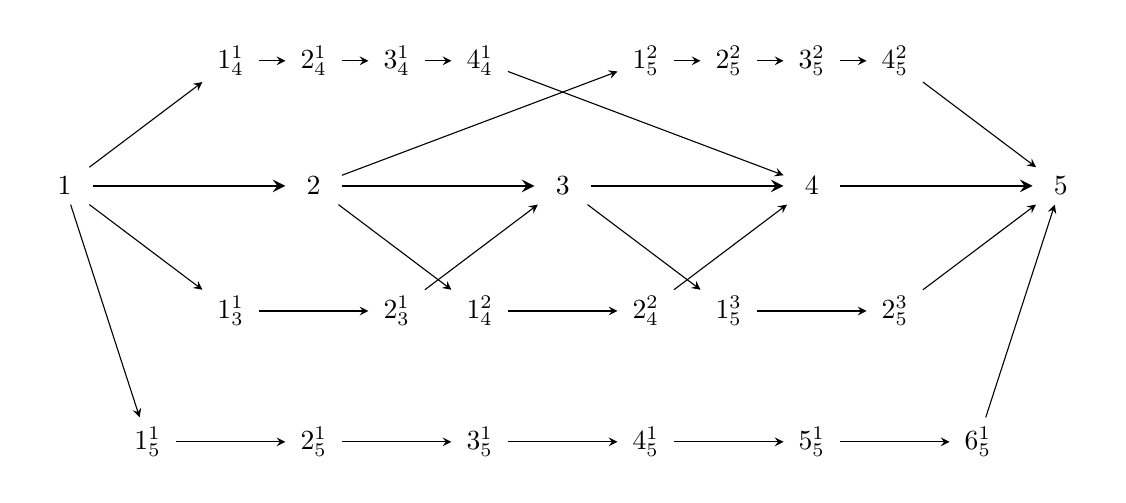
\begin{tikzpicture}
    [
    point/.style={circle,draw,inner sep=0pt,minimum size=2mm},
    collection/.style={thick,rectangle,draw,inner sep=0pt,minimum height=14mm, minimum width= 9mm}
    ]
	  \matrix (m) [matrix of math nodes,row sep=3em,column sep=1em,minimum width=2em]
	  {   & & 1^1_4 & 2^1_4 & 3^1_4 & 4^1_4 & & 1^2_5 & 2^2_5 & 3^2_5 & 4^2_5 & & \\
	  	1 & & & 2 & & & 3 & & & 4 & & & 5 \\
	  	  & & 1^1_3 & & 2^1_3 & 1^2_4 & & 2^2_4 & 1^3_5 & & 2^3_5 & & \\
		  & 1^1_5 & & 2^1_5 & & 3^1_5 & & 4^1_5 & & 5^1_5 & & 6^1_5 & \\
		};
	  \path[-stealth]
	  	(m-1-3) edge (m-1-4)
		(m-1-4) edge (m-1-5)
		(m-1-5) edge (m-1-6)
		(m-1-6) edge (m-2-10)
		(m-1-8) edge (m-1-9)
		(m-1-9) edge (m-1-10)
		(m-1-10) edge (m-1-11)
		(m-1-11) edge (m-2-13)
	  	(m-2-1) edge [line width=1pt] (m-2-4)
				edge (m-3-3)
				edge (m-1-3)
				edge (m-4-2)
		(m-2-4) edge [line width=1pt] (m-2-7)
				edge (m-3-6)
				edge (m-1-8)
		(m-2-7) edge [line width=1pt] (m-2-10)
				edge (m-3-9)
		(m-2-10) edge [line width=1pt] (m-2-13)
		(m-3-3) edge (m-3-5)
		(m-3-5) edge (m-2-7)
		(m-3-6) edge (m-3-8)
		(m-3-8) edge (m-2-10)
		(m-3-9) edge (m-3-11)
		(m-3-11) edge (m-2-13)
		(m-4-2) edge (m-4-4)
		(m-4-4) edge (m-4-6)
		(m-4-6) edge (m-4-8)
		(m-4-8) edge (m-4-10)
		(m-4-10) edge (m-4-12)
		(m-4-12) edge (m-2-13)
	  ;
	\end{tikzpicture}
  \caption{Stretched Yablo}
  \label{fig:stretched_yablo}
\end{figure}
Shown above are parts of the Stretched Yablo-graph described.
We denote the core vertices by natural numbers.
The peripheral vertices contained in each path is denoted by $n^x_y$ where $x$ and $y$ is the source and target, respectively, of the path in which the vertex is contained.
$n$ denoted the relative position on the path.

Based on the given definition of Stretched Yablo and the notation from above, we get the following sets of axioms:
\begin{align}
  N1a &= \{\; \ol{x(x+1)} \;&&|\; x \in \mathbb{N} \; \} \\
	N1b &= \{\; \ol{x1^x_y} \;&&|\; x,y \in \mathbb{N}, x+1 < y \; \} \\
	N2 &= \{\; \ol{n^x_y(n+1)^x_y} \;&&|\; n,x,y \in \mathbb{N}, x+1 < y, n < 2(y-x) - 2 \; \} \\
	N3 &= \{\; \ol{(2(y-x)-1)^x_yy} \;&&|\; n,x,y \in \mathbb{N}, x+1 < y \; \} \\
	O1 &= \{\; x(x+1)1^x_{x+2}1^x_{x+3}\dots \;&&|\; x \in \mathbb{N} \; \} \\
  O2 &= \{\; n^x_y(n+1)^x_y \;&&|\; n,x,y \in \mathbb{N}, x+1 < y, n < 2(y-x) - 2 \; \} \\
	O3 &= \{\; (2(y-x)-1)^x_yy \;&&|\; n,x,y \in \mathbb{N}, x+1 < y \; \}
\end{align}
We get that NAND = $N1a \cup N1b \cup N2 \cup N3$ and that OR = $O1 \cup O2 \cup O3$.
One can identify the different axioms by looking at the figure above\footnote{recall how NANDs corresponds to edges, while ORs corresponds to vertices}:
$N1a$ are the edges making up the core ray of the graph, $N1b$ are the edges going from a core vertex onto a peripheral vertex, $N2$ are the edges between two peripheral vertices and $N3$ are the edges going from a peripheral vertex back onto a core vertex.
$O1$ are the vertices on the core ray, $O2$ and $O3$ are the peripheral vertices, $O3$ being the ones that points back to a core vertex.

In order to prove $\varnothing$ from these axiom, we prove some intermediate clauses.

	\pagebreak
	% !TEX root= ../main.tex
\externaldocument{../binary_nands/odd_vels}
\section{Provability of NAND-clauses from vels}
\label{sec:Provability of NAND-clauses from vels}
This section will prove the following statement:
Given a graph where two vertices $a$ and $b$ are connected by a vel, as defined in Section~\ref{sec:Odd vels}, the binary NAND-clause $\ol{ab}$ is provable in Neg.

Let $\mathbf{G} = (G,N)$ be a graph containing the vertices $a,b$ such that they have a vel between them.
By definition, this means that there exists a vertex $c$ such that there is an oddly trimmed path from $a$ to $c$ and from $b$ to $c$, one of odd length and one of even length.

Let $P$ and $Q$ be the two sets containing the vertices in the path from $a$ to $c$ and from $b$ to $c$, respectively.
We will denote each element of $P$ as $p_i$ where $i \in \mathbb{N}$ is the position of that vertex in the path, starting at 0.
The elements of $Q$ will be named $q_i$ by the same rule.
We immediately have that $a = p_0$ and $b = q_0$.
As long as the trimming restrictions are met, $P$ and $Q$ might overlap, i.e. we might have cases where $p_j = q_k$ from some $i$ and $j$.

We assume, without any loss of generality, that the path from $a$ to $c$ is of odd length, making the path from $b$ to $c$.
We denote the lengths of the two paths by the numbers $n$ and $m$, giving us that $c = p_n = q_m$.
The path from $b$ to $c$ might also be empty, making $b = p_0 = c$.

\begin{figure}[!h]
  \centering
  \begin{tikzpicture}
    [
    point/.style={circle,draw,inner sep=0pt,minimum size=2mm}
    ]
    \node (a) at (0,5) [point, label=left:${a = p_0}$] {};
    \node (p1) at (1,4) [point, label=left:$p_1$] {};
    \node (pd) at (2,3) [] {$\dots$};
    \node (pn2) at (3,2) [point, label=left:$p_{n-2}$] {};
    \node (pn1) at (4,1) [point, label=left:$p_{n-1}$] {};
    \node (c) at (5,0) [point, label=right:${c = p_n = q_m}$] {};
    \node (qm1) at (6,1) [point, label=right:$q_{m-1}$] {};
    \node (qm2) at (7,2) [point, label=right:$q_{m-2}$] {};
    \node (qd) at (8,3) [] {$\dots$};
    \node (q1) at (9,4) [point, label=right:$q_1$] {};
    \node (b) at (10,5) [point, label=right:${b = q_0}$] {};
    \draw [-latex] (a) to (p1);
    \draw [-latex] (p1) to (pd);
    \draw [-latex] (pd) to (pn2);
    \draw [-latex] (pn2) to (pn1);
    \draw [-latex] (pn1) to (c);
    \draw [-latex] (b) to (q1);
    \draw [-latex] (q1) to (qd);
    \draw [-latex] (qd) to (qm2);
    \draw [-latex] (qm2) to (qm1);
    \draw [-latex] (qm1) to (c);

    \node (e1) [below left=6mm and 4mm of c]  {};
    \node (e2) [below=8mm of c] {};
    \node (e3) [below right=6mm and 4mm of c] {};
    \draw [dashed] (e1) to (c);
    \draw [dashed] (e2) to (c);
    \draw [dashed] (e3) to (c);

    \node (ba) [below left=6mm and 4mm of a] {};
    \node (bn1) [below left=6mm and 4mm of pn1] {};
    \node (bb) [below right=6mm and 4mm of b] {};
    \node (bm2) [below right=6mm and 4mm of qm2] {};
    \draw [dashed] (ba) to (a);
    \draw [dashed] (bn1) to (pn1);
    \draw [dashed] (bb) to (b);
    \draw [dashed] (bm2) to (qm2);
  \end{tikzpicture}
  \caption{A general vel between $a$ and $b$}
  \label{fig:general_odd_vel}
\end{figure}

  \pagebreak
  % !TEX root= ../main.tex
\section{Axioms in Neg proofs}
\label{sec:Axioms in Neg proofs}

	\pagebreak
	\printbibliography
\end{document}
